\pdfpagewidth = 8.5in
\pdfpageheight = 11.0in
\usepackage[left=1in,right=1in,top=1in,bottom=1in]{geometry}

\pagestyle{plain}
\pagenumbering{arabic}
\usepackage{setspace}
\usepackage[usenames]{color}
\usepackage[fleqn]{amsmath}
\usepackage{amssymb}
\usepackage{graphicx}
\usepackage{url}
\usepackage{verbatim}
\usepackage{appendix}
\usepackage{indentfirst}
\usepackage{booktabs}
\usepackage{multirow}
\usepackage[table, x11names]{xcolor}
\usepackage{ragged2e}
\usepackage{upgreek}
\usepackage{lscape}
\usepackage{longtable}
\usepackage[flushleft, referable]{threeparttablex}
\usepackage{rotating}
\usepackage[T1]{fontenc}
\usepackage[titles]{tocloft}
\usepackage{xspace}
\usepackage{ifthen}
\usepackage{cancel}
\usepackage{rotating}
\usepackage{array}
\usepackage{tabulary}
\usepackage{authblk}

\usepackage{hyperref}
\hypersetup{pdfborder={0 0 0}, colorlinks=true, urlcolor=black, linkcolor=black, citecolor=black}
\usepackage[capitalize]{cleveref}
\newcommand{\crefrangeconjunction}{--}

\usepackage[right, mathlines]{lineno}
\setlength\linenumbersep{1cm}
\def\linenumberfont{\normalfont\scriptsize\sffamily}

% \usepackage[format=plain, labelsep=period, justification=raggedright, singlelinecheck=true, skip=2pt, font=sf]{caption}
\usepackage{caption}
\DeclareCaptionLabelFormat{noSpace}{{#1}{#2}}
\DeclareCaptionListFormat{figList}{Figure {#2}.}
\DeclareCaptionListFormat{sFigList}{Figure S{#2}.}
\usepackage{subfig}

%\DeclareMathSizes{12}{12}{7}{5}

% \usepackage[round]{natbib}

% \makeatletter
%   \renewcommand{\section}{\@startsection{section}{1}{0mm}%
%     {-12pt}%
%     {12pt}%
%     {\sffamily\LARGE\itshape}}
% \makeatother

% \makeatletter
%   \renewcommand{\subsection}{\@startsection{subsection}{1}{0mm}%
%   {-10pt}%
%   {4pt}%
%   {\sffamily\large\bfseries\MakeUppercase}}
% \makeatother

% \makeatletter
%   \renewcommand{\subsubsection}{\@startsection{subsubsection}{1}{0mm}%
%   {-10pt}%
%   {10pt}%
%   {\sffamily\large\itshape}}
% \makeatother

% make list of figures ragged right
% \makeatletter
%   \renewcommand{\@tocrmarg}{0cm plus1fil}
% \makeatother

\setlength\linenumbersep{1cm}

% \newcommand{\change}[1]{{\color{blue} #1}\xspace}
\newcommand{\change}[1]{{\color{black} #1}\xspace}


\newcommand{\citationNeeded}{\textcolor{magenta}{\textbf{[CITATION NEEDED!]}}\xspace}
\newcommand{\tableNeeded}{\textcolor{magenta}{\textbf{[TABLE NEEDED!]}}\xspace}
\newcommand{\figureNeeded}{\textcolor{magenta}{\textbf{[FIGURE NEEDED!]}}\xspace}
\newcommand{\highLight}[1]{\textcolor{magenta}{\MakeUppercase{#1}}}

\newcommand{\editorialNote}[1]{\textcolor{red}{[\textit{#1}]}}
\newcommand{\ignore}[1]{}
\newcommand{\addTail}[1]{\textit{#1}.---}
\newcommand{\super}[1]{\ensuremath{^{\textrm{#1}}}}
\newcommand{\sub}[1]{\ensuremath{_{\textrm{#1}}}}
\newcommand{\dC}{\ensuremath{^\circ{\textrm{C}}}}

\providecommand{\e}[1]{\ensuremath{\times 10^{#1}}}

\newcommand{\mthnote}[2]{{\color{red} #2}\xspace}
\newcommand{\cwlnote}[2]{{\color{orange} #2}\xspace}

\newcommand{\ifTwoArgs}[3]{\ifthenelse{\equal{#1}{}\or\equal{#2}{}}{}{#3}\xspace}
\newcommand{\ifArg}[2]{\ifthenelse{\equal{#1}{}}{}{#2}\xspace}

%% New notation for divergence times
\newcommand{\divTime}[1]{\ensuremath{\tau_{#1}}\xspace}
\newcommand{\divTimeVector}{\ensuremath{\boldsymbol{\divTime{}}}\xspace}
\newcommand{\divTimeIndex}[1]{\ensuremath{t_{#1}}\xspace}
\newcommand{\divTimeIndexVector}{\ensuremath{\mathbf{\divTimeIndex{}}}\xspace}
\newcommand{\divTimeMap}[1]{\ensuremath{T_{#1}}\xspace}
\newcommand{\divTimeMapVector}{\ensuremath{\mathbf{\divTimeMap{}}}\xspace}
\newcommand{\divTimeScaled}[2]{\ensuremath{\mathcal{T}_{#1\protect\ifTwoArgs{#1}{#2}{,}#2}}\xspace}
\newcommand{\divTimeScaledVector}{\ensuremath{\mathbf{\divTimeScaled{}{}}}\xspace}
\newcommand{\divTimeMean}{\ensuremath{\bar{\divTimeMap{}}}\xspace}
\newcommand{\divTimeVar}{\ensuremath{s^{2}_{\divTimeMap{}}}\xspace}
\newcommand{\divTimeDispersion}{\ensuremath{D_{\divTimeMap{}}}\xspace}
\newcommand{\divTimeNum}{\ensuremath{\lvert \divTimeVector \rvert}\xspace}
\newcommand{\demographicParams}[1]{\ensuremath{\Theta_{#1}}\xspace}
\newcommand{\demographicParamVector}{\ensuremath{\mathbf{\demographicParams{}}}\xspace}
\newcommand{\popSampleSize}[2]{\ensuremath{n_{#1\protect\ifTwoArgs{#1}{#2}{,}#2}}}
\newcommand{\gammaShape}[1]{\ensuremath{a_{#1}}\xspace}
\newcommand{\gammaScale}[1]{\ensuremath{b_{#1}}\xspace}
\newcommand{\betaA}[1]{\ensuremath{a_{#1}}\xspace}
\newcommand{\betaB}[1]{\ensuremath{b_{#1}}\xspace}
\newcommand{\integerPartitionSet}[1]{\ensuremath{a({#1})}\xspace}
\newcommand{\integerPartitionNum}[1]{\ensuremath{\lvert \integerPartitionSet{#1} \rvert}\xspace}
\newcommand{\concentrationParam}{\ensuremath{\chi}\xspace}
\newcommand{\stirlingFirst}[2]{\ensuremath{c(#1, #2)}\xspace}
\newcommand{\descendantThetaMean}[1]{\ensuremath{\bar{\theta}_{D\protect\ifArg{#1}{,}#1}}\xspace}
\newcommand{\numPriorSamples}{\ensuremath{\mathbf{n}}\xspace}
\newcommand{\paramSampleVector}[1]{\ensuremath{\Lambda_{#1}}\xspace}
\newcommand{\paramSampleMatrix}{\ensuremath{\boldsymbol{\paramSampleVector{}}}\xspace}
\newcommand{\modelDPP}{\ensuremath{M_{DPP}}\xspace}
\newcommand{\modelDPPOrdered}{\ensuremath{M^{\circ}_{DPP}}\xspace}
\newcommand{\modelUniform}{\ensuremath{M_{Uniform}}\xspace}
\newcommand{\modelUshaped}{\ensuremath{M_{Ushaped}}\xspace}
\newcommand{\modelOld}{\ensuremath{M_{msBayes}}\xspace}
\newcommand{\priorDPP}[1]{\ensuremath{DP(\concentrationParam #1)}\xspace}
\newcommand{\priorUniform}{\ensuremath{DU\{\integerPartitionSet{\npairs{}}\}}\xspace}
\newcommand{\priorOld}{\ensuremath{DU\{1, \ldots, \npairs{}\}}\xspace}
\newcommand{\powerSeriesOld}{\ensuremath{\mathcal{M}_{msBayes}}\xspace}
\newcommand{\powerSeriesUniform}{\ensuremath{\mathcal{M}_{Uniform}}\xspace}
\newcommand{\powerSeriesExp}{\ensuremath{\mathcal{M}_{Exp}}\xspace}

\newcommand{\allDatasets}{\ensuremath{\mathcal{\alignment{}{}}}\xspace}
\newcommand{\allParameterValues}{\ensuremath{\boldsymbol{\Theta}}\xspace}
\newcommand{\bayesfactor}[2]{\ensuremath{BF_{#1\protect\ifArg{#2}{,}#2}}}
\newcommand{\given}{\ensuremath{\,|\,}\xspace}
\newcommand{\msb}{\upshape\texttt{\MakeLowercase{ms\MakeUppercase{B}ayes}}\xspace}
\newcommand{\abctoolbox}{\upshape\texttt{ABCtoolbox}\xspace}
\newcommand{\dppmsbayes}{\upshape\texttt{dpp-msbayes}\xspace}
\newcommand{\pymsbayes}{\upshape\texttt{PyMsBayes}\xspace}
\newcommand{\hky}{HKY85\xspace}
\newcommand{\uniformMin}[1]{\ensuremath{a_{#1}}\xspace}
\newcommand{\uniformMax}[1]{\ensuremath{b_{#1}}\xspace}
\newcommand{\locusRateHetShapeParameter}{\ensuremath{\alpha}\xspace}
\newcommand{\ancestralThetaVector}{\ensuremath{\boldsymbol{\theta_{A}}}\xspace}
\newcommand{\descendantThetaVector}[1]{\ensuremath{\boldsymbol{\theta_{D#1}}}\xspace}
\newcommand{\divtscaledvector}{\ensuremath{\mathbf{{\divtscaled{}{}}}}\xspace}
\newcommand{\divtvector}{\ensuremath{\boldsymbol{\divt{}}}\xspace}
\newcommand{\divtuniquevector}{\ensuremath{\mathbf{\divtunique{}}}\xspace}
\newcommand{\bottleTimeVector}{\ensuremath{\boldsymbol{\bottleTime{}}}\xspace}
\newcommand{\bottleTime}[1]{\ensuremath{\divt{B\ifArg{#1}{,}#1}}\xspace}
\newcommand{\bottleScalarVector}[1]{\ensuremath{\boldsymbol{\bottleScalar{#1}{}}}\xspace}
\newcommand{\bottleScalar}[2]{\ensuremath{\zeta_{D#1\protect\ifArg{#2}{,}#2}}\xspace}
\newcommand{\migrationRateVector}{\ensuremath{\mathbf{\migrationRate{}}}\xspace}
\newcommand{\geneTreeVector}{\ensuremath{\mathbf{\geneTree{}{}}}\xspace}
\newcommand{\alignmentVector}{\ensuremath{\mathbf{\alignment{}{}}}\xspace}
\newcommand{\alignment}[2]{\ensuremath{X_{#1\protect\ifTwoArgs{#1}{#2}{,}#2}}\xspace}
\newcommand{\geneTree}[2]{\ensuremath{G_{#1\protect\ifTwoArgs{#1}{#2}{,}#2}}\xspace}
\newcommand{\migrationRate}[1]{\ensuremath{m_{#1}}\xspace}
\newcommand{\recombinationRate}{\ensuremath{r}\xspace}
\newcommand{\ploidyScalar}[2]{\ensuremath{\rho_{#1\protect\ifTwoArgs{#1}{#2}{,}#2}}\xspace}
\newcommand{\ploidyScalarVector}{\ensuremath{\boldsymbol{\ploidyScalar{}{}}}\xspace}
\newcommand{\descendantRelativeThetaVector}[1]{\ensuremath{\boldsymbol{\eta_{D#1}}}\xspace}
\newcommand{\descendantRelativeTheta}[2]{\ensuremath{\eta_{D#1\protect\ifArg{#2}{,}#2}}\xspace}
\newcommand{\mutationRateScalarConstant}[2]{\ensuremath{\nu_{#1\protect\ifTwoArgs{#1}{#2}{,}#2}}\xspace}
\newcommand{\mutationRateScalarConstantVector}{\ensuremath{\boldsymbol{\mutationRateScalarConstant{}{}}}\xspace}
\newcommand{\locusMutationRateScalar}[1]{\ensuremath{\upsilon_{#1}}\xspace}
\newcommand{\locusMutationRateScalarVector}{\ensuremath{\boldsymbol{\upsilon}}\xspace}
\newcommand{\hkyModel}[2]{\ensuremath{\phi_{#1\protect\ifTwoArgs{#1}{#2}{,}#2}}\xspace}
\newcommand{\hkyModelVector}{\ensuremath{\boldsymbol{\hkyModel{}{}}}\xspace}
\newcommand{\mutationRate}{\ensuremath{\mu}\xspace}
\newcommand{\iid}{\textit{iid}\xspace}
\newcommand{\model}[1]{\ensuremath{\Theta}\xspace}
\newcommand{\npairs}[1]{\ensuremath{Y_{#1}}}
\newcommand{\nloci}[1]{\ensuremath{k_{#1}}\xspace}
\newcommand{\nlociTotal}{\ensuremath{K}\xspace}
\newcommand{\myTheta}[1]{\ensuremath{\theta_{#1}}}
\newcommand{\ancestralTheta}[1]{\ensuremath{\theta_{A\protect\ifArg{#1}{,}#1}}\xspace}
\newcommand{\descendantTheta}[2]{\ensuremath{\theta_{D#1\protect\ifArg{#2}{,}#2}}\xspace}
\newcommand{\meanDescendantTheta}[1]{\ensuremath{\descendantTheta{}{#1}}\xspace}
\newcommand{\nucdiv}[1]{\ensuremath{\pi_{#1}}}

\newcommand{\ssVector}[1]{\ensuremath{\mathbf{\alignmentSS{#1}{}}}\xspace}
\newcommand{\ssVectorObs}{\ensuremath{\ssVector{}^*}\xspace}
\newcommand{\ssSpace}{\ensuremath{\euclideanSpace{\ssVectorObs}}\xspace}
\newcommand{\ssVectorObsPLS}{\ensuremath{\ssVectorObs_{PLS}}\xspace}
\newcommand{\alignmentSS}[2]{\ensuremath{S_{#1\protect\ifTwoArgs{#1}{#2}{,}#2}}\xspace}
\newcommand{\alignmentSSObs}[2]{\ensuremath{\alignmentSS{#1}{#2}^*}\xspace}
\newcommand{\tol}{\ensuremath{\epsilon}\xspace}
\newcommand{\euclideanSpace}[1]{\ensuremath{B_{\tol}(#1)}\xspace}
\newcommand{\hpvector}[1]{\ensuremath{\Lambda_{#1}}}
\newcommand{\divtscaled}[2]{\ensuremath{t_{#1\protect\ifTwoArgs{#1}{#2}{,}#2}}}
\newcommand{\divt}[1]{\ensuremath{\tau_{#1}}}
\newcommand{\divtunique}[1]{\ensuremath{T_{#1}}}
\newcommand{\ssMatrix}{\ensuremath{\mathbb \alignmentSS{}{}}\xspace}
\newcommand{\ssMatrixRaw}[1]{\ensuremath{{\ssMatrix}_{stats#1}}\xspace}
\newcommand{\ssMatrixPLS}[1]{\ensuremath{{\ssMatrix}_{PLS#1}}\xspace}
\newcommand{\hpmatrix}[1]{\ensuremath{\mathcal{P}_{#1}}}
\newcommand{\meant}[2]{\ensuremath{E(\divt{#1})_{#2}}}
\newcommand{\meantestimate}{\ensuremath{\hat{E(\divt{})}}\xspace}
\newcommand{\vart}[2]{\ensuremath{Var(\divt{#1}{})_{#2}}}
\newcommand{\vmratio}[1]{\ensuremath{\Omega_{#1}}}
\newcommand{\numt}[1]{\ensuremath{\Psi_{#1}}}
\newcommand{\probnumt}[2]{\ensuremath{p(\numt{#1} = {#2})}}
\newcommand{\postprobnumt}[1]{\ensuremath{p(\numt{} = {#1}|\ssSpace)}}
\newcommand{\postprobnumtnot}[1]{\ensuremath{p(\numt{} \neq {#1}|\ssSpace)}}
\newcommand{\postprobomegasimult}{\ensuremath{p(\vmratio{} < 0.01 | \ssSpace)}\xspace}
\newcommand{\modelprior}[1]{\ensuremath{f(\model{})}}
\newcommand{\modelpost}[1]{\ensuremath{f(\model{}|\ssSpace)}}
\newcommand{\npriorsamples}{\ensuremath{n}\xspace}
\newcommand{\globalcoalunit}{\ensuremath{4\globalpopsize}\xspace}
\newcommand{\globalpopsize}{\ensuremath{N_C}\xspace}
\newcommand{\effectivePopSize}[1]{\ensuremath{N_e{#1}}\xspace}
\newcommand{\coalunit}{\ensuremath{4\effectivePopSize{}}\xspace}
\newcommand{\priorsample}[1]{\ensuremath{\hpmatrix{\modelprior{}}}}
\newcommand{\truncprior}[1]{\ensuremath{\hpmatrix{\tol}}\xspace}
\newcommand{\postsample}[1]{\ensuremath{\hpmatrix{\modelpost{}}}}
\newcommand{\abcllr}[1]{ABC\sub{LLR}}
\newcommand{\abcglm}[1]{ABC\sub{GLM}}
\newcommand{\integerPartition}[1]{\ensuremath{a({#1})}}
\newcommand{\uniqueModel}[2]{\ensuremath{M_{#1\protect\ifTwoArgs{#1}{#2}{,}#2}}}
\newcommand{\taxonLocusVector}[1]{\ensuremath{\{#1{1}{1},\ldots,#1{\npairs{}}{\nloci{\npairs{}}}\}}\xspace}
\newcommand{\taxonVector}[1]{\ensuremath{\{#1{1},\ldots,#1{\npairs{}}\}}\xspace}
\newcommand{\locusVector}[1]{\ensuremath{\{#1{1},\ldots,#1{\nlociTotal}\}}\xspace}

\newcommand{\validationAccuracyCaption}[2]{Estimation accuracy for model
    #2 when analyzing data generated under #1.
    A random sample of 5000 posterior estimates (from 50,000) are plotted,
    including both (A, B, \& C) unadjusted and (D, E, \&
    F) GLM-regression-adjusted estimates.
    Normal random variates ($N(0, 0.005)$) have been added to the estimates and
    true values of \divTimeNum (A \& D) to reduce overlap of plot symbols.
    The root mean square error (RMSE) calculated from the 5000 estimates is
    provided.}
\newcommand{\validationModelChoiceCaption}[2]{Model-choice accuracy for model
    #2 when analyzing data generated under #1.
    The estimated posterior probability of a single divergence event, based on
    (A \& C) $\divTimeNum = 1$ and (B \& D) $\divTimeDispersion < 0.01$, from
    50,000 posterior estimates are assigned to bins of width 0.05 and plotted
    against the proportion of replicates in each bin where the truth is
    $\divTimeNum = 1$ or $\divTimeDispersion < 0.01$.
    Results based on the (A \& B) unadjusted and (C \& D) GLM-adjusted
    posterior estimates are shown.}
\newcommand{\powerAccuracyCaption}[2]{Estimation accuracy for model
    #2 when analyzing data generated under the series of models #1.
    The true versus estimated value of the dispersion index of divergence
    times (\divTimeDispersion) is plotted for 1000 datasets simulated
    under each of the #1 models, and the proportion of estimates less
    than the truth, $p(\hat{\divTimeDispersion} < \divTimeDispersion)$,
    is shown for each data model.}
\newcommand{\powerPsiCaption}[2]{
    The power of model #2 to detect random variation in divergence times as
    simulated under the series of models #1.
    The plots illustrate the estimated number of divergence events
    ($\hat{\divTimeNum}$) from analyses of 1000 datasets simulated under each
    of the #1 models, with the the estimated probability of the model inferring
    one divergence event, $p(\hat{\divTimeNum} = 1)$, given for each data
    model.}
\newcommand{\powerDispersionCaption}[2]{
    The power of model #2 to detect random variation in divergence times as
    simulated under the series of models #1.
    The plots illustrate the estimated dispersion index of divergence times
    ($\hat{\divTimeDispersion}$) from analyses of 1000 datasets simulated under
    each of the #1 models, with the the estimated probability of the model
    inferring one divergence event, $p(\hat{\divTimeDispersion} < 0.01)$, given
    for each data model.}
\newcommand{\powerPsiProbCaption}[2]{
    The tendency of model #2 to support one divergence event when there is
    random variation in divergence times as simulated under the series of
    models #1.
    The plots illustrate histograms of the estimated posterior probability of
    the one divergence model, $p(\divTimeNum = 1 | \ssSpace)$, from analyses of
    1000 datasets simulated under each of the #1 models, with the the estimated
    probability of the model strongly supporting one divergence event,
    $p(BF_{\divTimeNum = 1, \divTimeNum \neq 1} > 10)$, given for each data
    model.}
\newcommand{\powerDispersionProbCaption}[2]{
    The tendency of model #2 to support one divergence event when there is
    random variation in divergence times as simulated under the series of
    models #1.
    The plots illustrate histograms of the estimated posterior probability of
    the one divergence model, $p(\divTimeDispersion < 0.01 | \ssSpace)$, from
    analyses of 1000 datasets simulated under each of the #1 models, with the
    the estimated probability of the model strongly supporting one divergence
    event, $p(BF_{\divTimeDispersion < 0.01, \divTimeDispersion \geq 0.01} >
    10)$, given for each data model.}
\newcommand{\simulationDescription}[2]{\change{Each plot represents #1
    simulation replicates using the same $#2$ samples from the prior}}
\newcommand{\simulationDistribution}{\ensuremath{\divt{} \sim U(0,
    \divt{max})}\xspace}
\newcommand{\estimateDescription}[2]{All estimates were obtained using #1 and #2}
\newcommand{\estimateDescriptionUncorrected}[1]{All estimates based on
    unadjusted posterior, \truncprior{}, obtained using #1}
\newcommand{\priorDescription}[4]{Prior settings were \priorSettings{#1}{#2}{#3}{#4}}
\newcommand{\priorSettings}[4]{$\divt{} \sim U(0, #1)$,
    $\meanDescendantTheta{} \sim U(#2, #3)$, and
    $\ancestralTheta{}{} \sim U(#2, #4)$}
\newcommand{\priorDescriptionBug}[4]{Prior settings were
    \priorSettingsBug{#1}{#2}{#3}{#4}}
\newcommand{\priorSettingsBug}[4]{$\divt{} \sim U(0, #1)$,
    $\meanDescendantTheta{} \sim U(#2, #3)$, and
    $\ancestralTheta{}{} \sim U(0.01, #4)$}
\newcommand{\simulationScheme}{simulations where \divt{} (in \globalcoalunit
    generations) for 22 population pairs is drawn from a series of uniform
    distributions, \simulationDistribution}
\newcommand{\captionPowerOmega}{Histograms of the estimated dispersion index
    of divergence times ($\hat{\vmratio{}}$) from \simulationScheme.
    The threshold for one divergence event \citep{Hickerson2006} is indicated
    by the dashed line, and the estimated probability of inferring one
    divergence event, $p(\hat{\vmratio{}}\le 0.01)$, is given for each
    \divt{max}}
\newcommand{\captionPowerPsiMode}{Histograms of the estimated number of
    divergence events ($\hat{\numt{}}$) from \simulationScheme.
    The estimated probability of inferring one divergence event,
    $p(\hat{\numt{}} = 1)$, is given for each \divt{max}}
\newcommand{\captionPowerPsi}{Histograms of the estimated posterior
    probability of one divergence event, \postprobnumt{1}, from
    \simulationScheme.
    The estimated probability of inferring one divergence event with a
    Bayes factor greater than 10 (dashed black line),
    $p(\bayesfactor{\numt{}=1}{\numt{} \ne 1} > 10)$, is given for each \divt{max}.
    The red line indicates $\postprobnumt{1} = 0.95$, and the estimated
    probability of inferring a posterior probability greater than 0.95 is given
    to the right of the line.}
\newcommand{\captionAccuracy}[1]{Accuracy and precision of #1 estimates from
    \simulationScheme.
    The proportion of estimates less than the true value ($p(\hat{#1}<#1)$) is
    given for each \divt{max}}
\newcommand{\samplingErrorTableNote}{An estimate of 1.0 for a posterior probability
    is an artifact of sampling error}


\newcommand{\refAccuracyALL}[1]{\labelcref{fig_acc_t_ss_llr_bug,fig_acc_t_ss_glm_bug,fig_acc_t_pls_llr_bug,fig_acc_t_pls_glm_bug,fig_acc_o_ss_llr_bug,fig_acc_o_ss_glm_bug,fig_acc_o_pls_llr_bug,fig_acc_o_pls_glm_bug}}
\newcommand{\refAccuracySS}[1]{\labelcref{fig_acc_t_ss_llr_bug,fig_acc_t_ss_glm_bug,fig_acc_o_ss_llr_bug,fig_acc_o_ss_glm_bug}}
\newcommand{\refAccuracySSfull}[1]{\labelcref{fig_acc_t_ssfull_llr_bug,fig_acc_t_ssfull_glm_bug,fig_acc_o_ssfull_llr_bug,fig_acc_o_ssfull_glm_bug}}
\newcommand{\refSSfull}[1]{\labelcref{fig_acc_t_ssfull_llr_bug,fig_acc_t_ssfull_glm_bug,fig_acc_o_ssfull_llr_bug,fig_acc_o_ssfull_glm_bug,fig_pow_o_ssfull_llr_bug,fig_pow_o_ssfull_glm_bug,fig_pow_psi_modes_ssfull_glm_bug}}
\newcommand{\refSS}[1]{\labelcref{fig_acc_t_ss_llr_bug,fig_acc_t_ss_glm_bug,fig_acc_o_ss_llr_bug,fig_acc_o_ss_glm_bug,fig_pow_o_ss_llr_bug,fig_pow_o_ss_glm_bug,fig_pow_psi_ss}}
\newcommand{\refAccuracyPLS}[1]{\labelcref{fig_acc_t_pls_llr_bug,fig_acc_t_pls_glm_bug,fig_acc_o_pls_llr_bug,fig_acc_o_pls_glm_bug}}
\newcommand{\refAccuracySScorrected}[1]{\labelcref{fig_acc_t_ss_llr_bug,fig_acc_t_ss_glm_bug,fig_acc_o_ss_llr_bug,fig_acc_o_ss_glm_bug}}
\newcommand{\refAccuracyPLScorrected}[1]{\labelcref{fig_acc_t_pls_llr_bug,fig_acc_t_pls_glm_bug,fig_acc_o_pls_llr_bug,fig_acc_o_pls_glm_bug}}
\newcommand{\refAccuracyUncorrected}[1]{\labelcref{fig_acc_t_ss_unc,fig_acc_t_pls_unc,fig_acc_o_ss_unc,fig_acc_o_pls_unc}}
\newcommand{\refAccuracyCorrected}[1]{\labelcref{fig_acc_t_ss_llr_bug,fig_acc_t_ss_glm_bug,fig_acc_t_pls_llr_bug,fig_acc_t_pls_glm_bug,fig_acc_o_ss_llr_bug,fig_acc_o_ss_glm_bug,fig_acc_o_pls_llr_bug,fig_acc_o_pls_glm_bug}}
\newcommand{\refAccuracyGLM}[1]{\labelcref{fig_acc_t_ss_glm_bug,fig_acc_t_pls_glm_bug,fig_acc_o_ss_glm_bug,fig_acc_o_pls_glm_bug}}
\newcommand{\refAccuracyLLR}[1]{\labelcref{fig_acc_t_ss_llr_bug,fig_acc_t_pls_llr_bug,fig_acc_o_ss_llr_bug,fig_acc_o_pls_llr_bug}}
\newcommand{\refAccuracyOmega}[1]{\labelcref{fig_acc_o_ss_llr_bug,fig_acc_o_ss_glm_bug,fig_acc_o_pls_llr_bug,fig_acc_o_pls_glm_bug}}
\newcommand{\refAccuracyOmegaUncorrected}[1]{\labelcref{fig_acc_o_ss_unc,fig_acc_o_pls_unc}}
\newcommand{\refAccuracyOmegaCorrected}[1]{\labelcref{fig_acc_o_ss_llr_bug,fig_acc_o_ss_glm_bug,fig_acc_o_pls_llr_bug,fig_acc_o_pls_glm_bug}}
\newcommand{\refAccuracyTime}[1]{\labelcref{fig_acc_t_ss_llr_bug,fig_acc_t_ss_glm_bug,fig_acc_t_pls_llr_bug,fig_acc_t_pls_glm_bug}}

\newcommand{\tn}{\tabularnewline}

\newcommand{\widthFigure}[5]{\begin{figure}[htbp]
\begin{center}
    \includegraphics[width=#1\textwidth]{#2}
    \captionsetup{#3}
    \caption{#4}
    \label{#5}
    \end{center}
    \end{figure}}

\newcommand{\heightFigure}[5]{\begin{figure}[htbp]
\begin{center}
    \includegraphics[height=#1]{#2}
    \captionsetup{#3}
    \caption{#4}
    \label{#5}
    \end{center}
    \end{figure}}

\newcommand{\mFigure}[3]{\widthFigure{1.0}{#1}{listformat=figList}{#2}{#3}\clearpage}
\newcommand{\siFigure}[3]{\widthFigure{1.0}{#1}{name=Figure S, labelformat=noSpace, listformat=sFigList}{#2}{#3}\clearpage}


\newcommand{\allParameters}{\ensuremath{\theta}\xspace}
\bibliography{../../manuscripts/bib/references}

\title[Estimating shared history]{An Improved Approximate-Bayesian Method for Estimating Shared
Evolutionary History}

\author[J.\ Oaks]{
    Jamie R.\ Oaks\inst{1,2}
}
\institute[University of Washington]{
    \inst{1}%
        Department of Ecology and Evolutionary Biology, University of Kansas
    \and
    \inst{2}%
        Department of Biology, University of Washington
}

% \date{\today}
\date{June 21, 2014}

\begin{document}
\maketitle

% \begin{frame}
% \frametitle{Outline}
% \tableofcontents
% \end{frame}

% \section{Intro}
% \begin{frame}
% \frametitle{Table of Contents}
% \tableofcontents[currentsection]
% \end{frame}

{
\usebackgroundtemplate{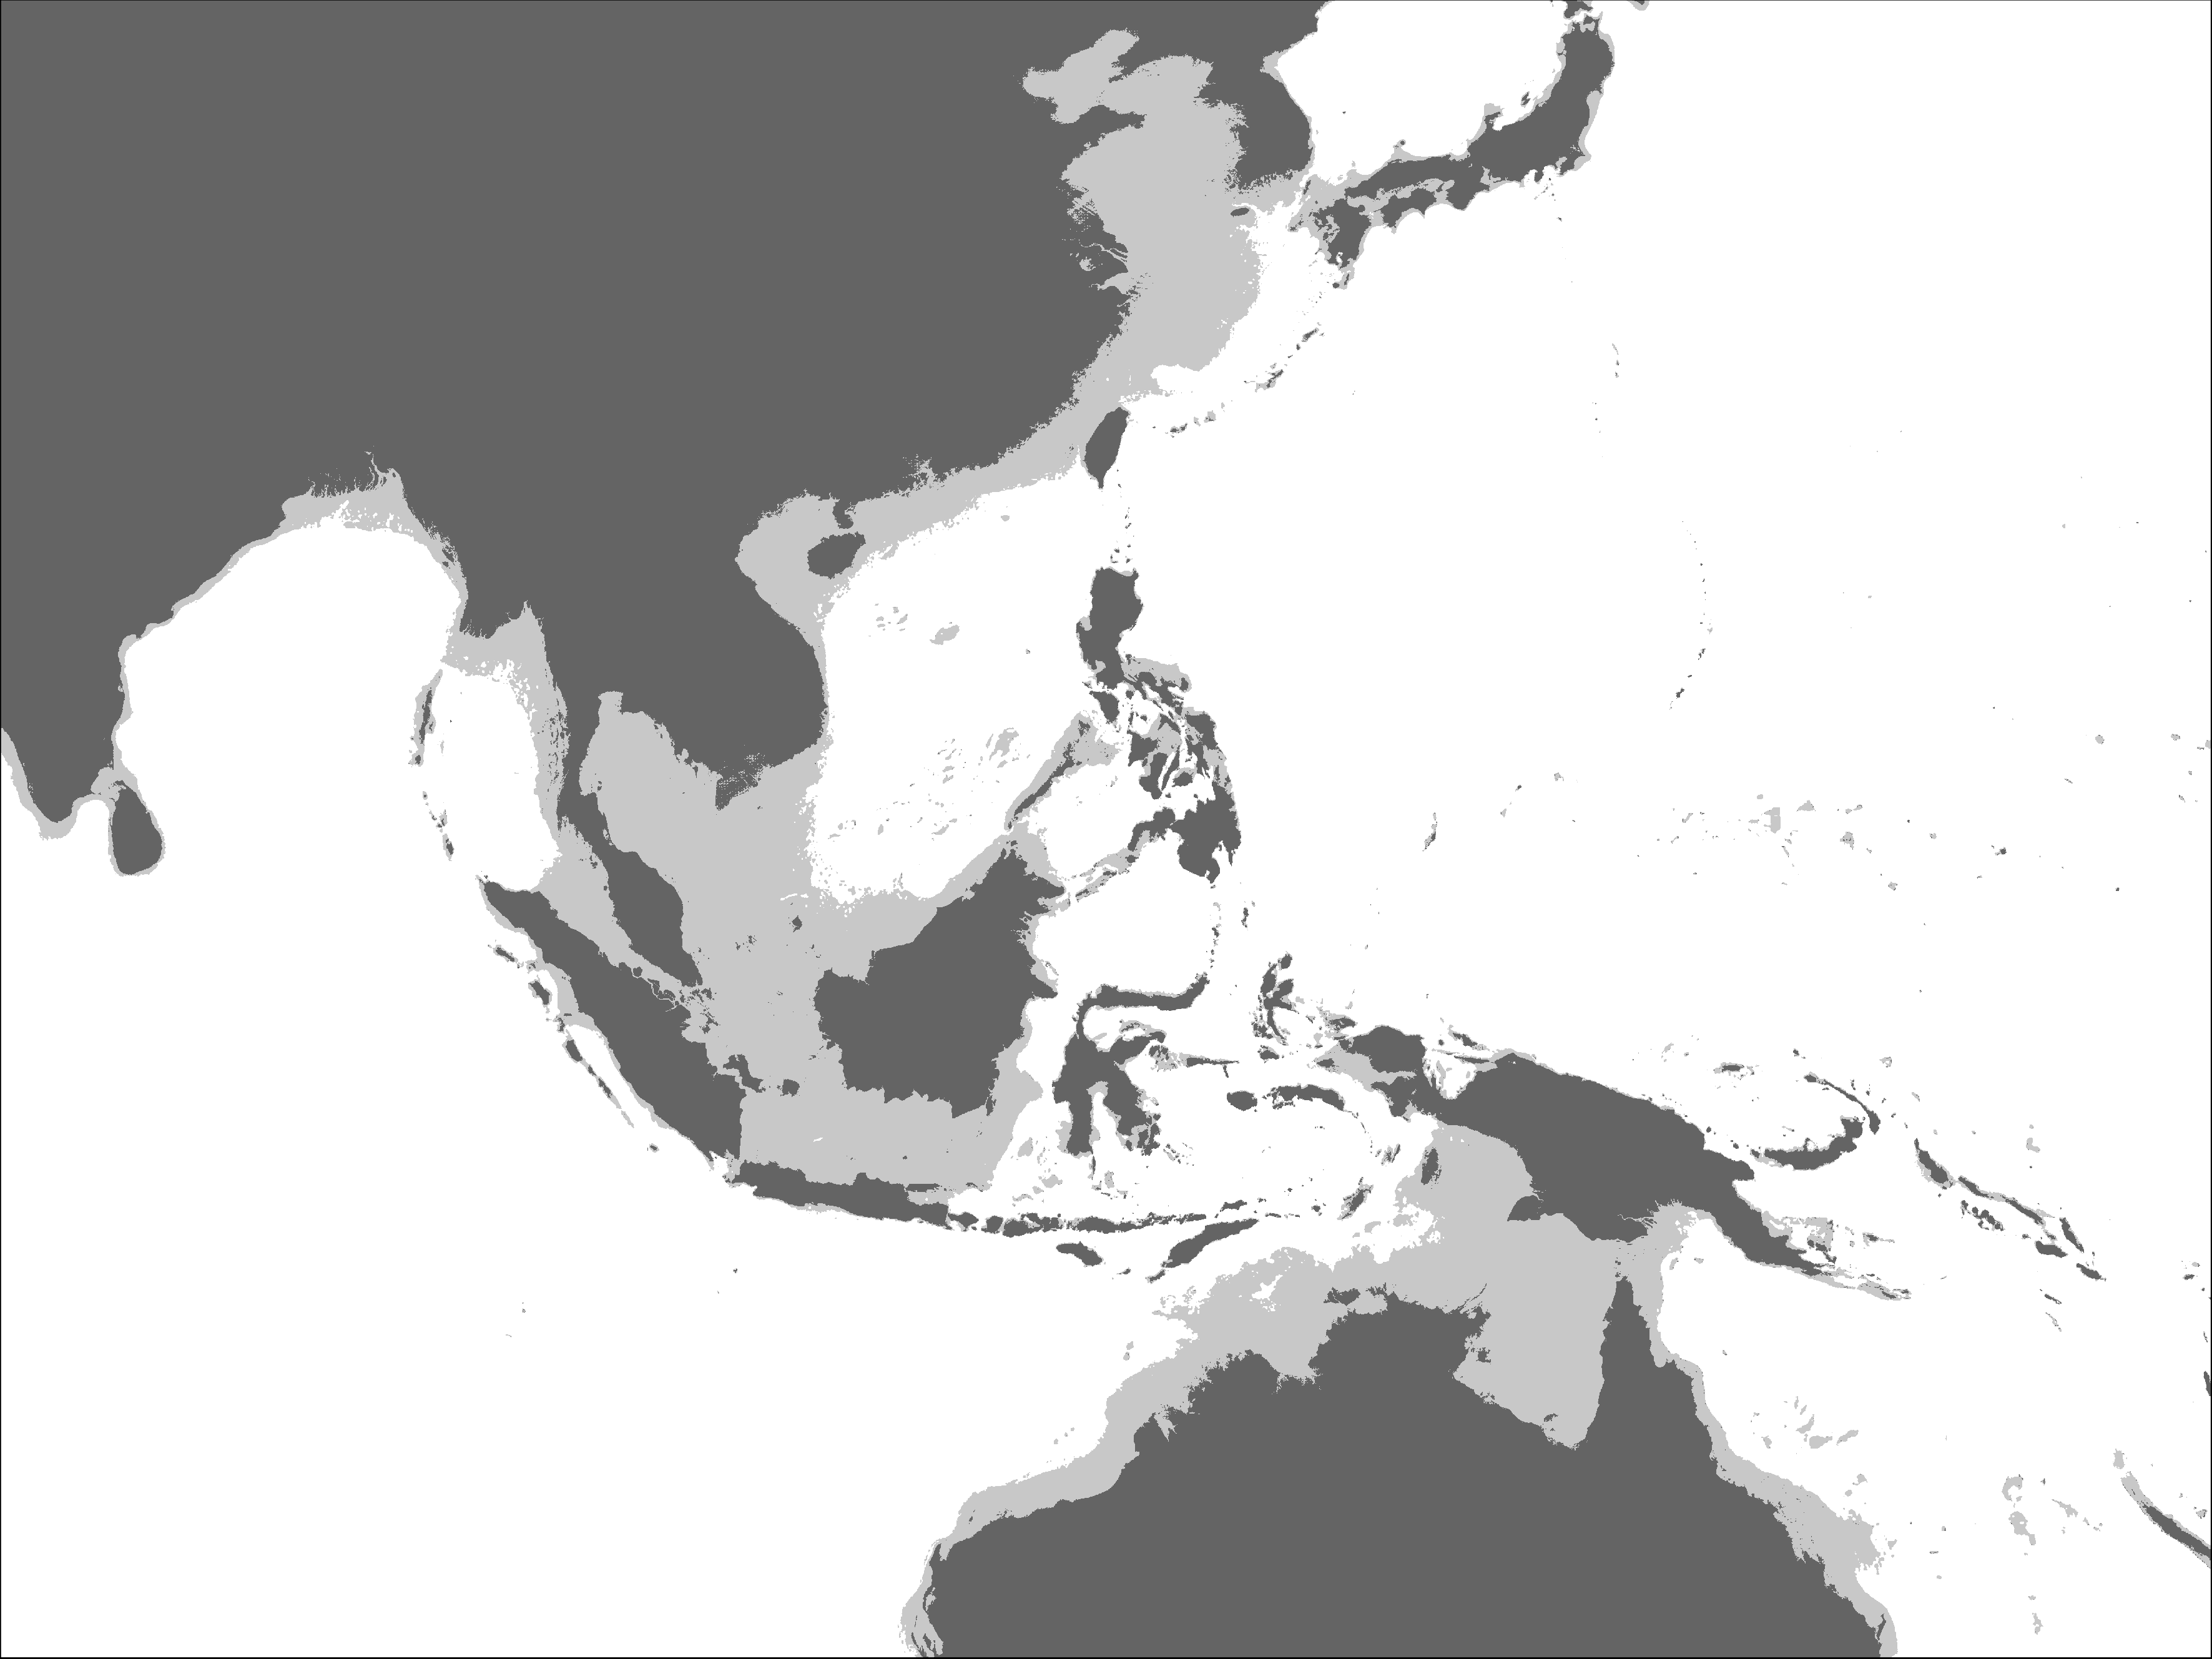
\includegraphics[width=\paperwidth]{../images/maps/se-asia-120.png}}
\begin{frame}
    \frametitle{Southeast Asia}    
\end{frame}
}

%TODO: NEED GENERAL INTRO

\begin{frame}
    \frametitle<1-6>{Community scale processes}
    \frametitle<7->{Divergence model choice}
    \begin{columns}[c]
        \column{.4\textwidth}
        \begin{onlyenv}<1-6>
            \begin{minipage}[c][0.5\textheight][c]{\linewidth}
            \end{minipage}
        \end{onlyenv}
        \begin{onlyenv}<7>
            \begin{minipage}[c][0.5\textheight][c]{\linewidth}
                \begin{displaybox}[0.95\linewidth]
                    \begin{minipage}[c][0.45\textheight][c]{0.95\linewidth}
                        \[
                            \divTimeMapVector = (\divTimeMap{1},\divTimeMap{2},\divTimeMap{3})
                        \]\vspace{0mm}
                        \[
                            model = 111
                        \]\vspace{0mm}
                        \[
                            \divTimeVector = \{\divTime{1}\}
                        \]\vspace{0mm}
                    \end{minipage}
                \end{displaybox}
            \end{minipage}
        \end{onlyenv}
        \begin{onlyenv}<8>
            \begin{minipage}[c][0.5\textheight][c]{\linewidth}
                \begin{displaybox}[0.95\linewidth]
                    \begin{minipage}[c][0.45\textheight][c]{0.95\linewidth}
                        \[
                            \divTimeMapVector = (260,260,260)
                        \]\vspace{0mm}
                        \[
                            model = 111
                        \]\vspace{0mm}
                        \[
                            \divTimeVector = \{260\}
                        \]\vspace{0mm}
                    \end{minipage}
                \end{displaybox}
            \end{minipage}
        \end{onlyenv}
        \begin{onlyenv}<9>
            \begin{minipage}[c][0.5\textheight][c]{\linewidth}
                \begin{displaybox}[0.95\linewidth]
                    \begin{minipage}[c][0.45\textheight][c]{0.95\linewidth}
                        \[
                            \divTimeMapVector = (397,260,260)
                        \]\vspace{0mm}
                        \[
                            model = 211
                        \]\vspace{0mm}
                        \[
                            \divTimeVector = \{260,397\}
                        \]\vspace{0mm}
                    \end{minipage}
                \end{displaybox}
            \end{minipage}
        \end{onlyenv}
        \begin{onlyenv}<10>
            \begin{minipage}[c][0.5\textheight][c]{\linewidth}
                \begin{displaybox}[0.95\linewidth]
                    \begin{minipage}[c][0.45\textheight][c]{0.95\linewidth}
                        \[
                            \divTimeMapVector = (260,397,260)
                        \]\vspace{0mm}
                        \[
                            model = 121
                        \]\vspace{0mm}
                        \[
                            \divTimeVector = \{260,397\}
                        \]\vspace{0mm}
                    \end{minipage}
                \end{displaybox}
            \end{minipage}
        \end{onlyenv}
        \begin{onlyenv}<11>
            \begin{minipage}[c][0.5\textheight][c]{\linewidth}
                \begin{displaybox}[0.95\linewidth]
                    \begin{minipage}[c][0.45\textheight][c]{0.95\linewidth}
                        \[
                            \divTimeMapVector = (260,260,397)
                        \]\vspace{0mm}
                        \[
                            model = 112
                        \]\vspace{0mm}
                        \[
                            \divTimeVector = \{260,397\}
                        \]\vspace{0mm}
                    \end{minipage}
                \end{displaybox}
            \end{minipage}
        \end{onlyenv}
        \begin{onlyenv}<12>
            \begin{minipage}[c][0.5\textheight][c]{\linewidth}
                \begin{displaybox}[0.95\linewidth]
                    \begin{minipage}[c][0.45\textheight][c]{0.95\linewidth}
                        \[
                            \divTimeMapVector = (260,95,397)
                        \]\vspace{0mm}
                        \[
                            model = 123
                        \]\vspace{0mm}
                        \[
                            \divTimeVector = \{260,95,397\}
                        \]\vspace{0mm}
                    \end{minipage}
                \end{displaybox}
            \end{minipage}
        \end{onlyenv}
        \begin{onlyenv}<13>
            \begin{minipage}[c][0.5\textheight][c]{\linewidth}
                \begin{displaybox}[0.95\linewidth]
                    \begin{minipage}[c][0.45\textheight][c]{0.95\linewidth}
                        \[
                            \divTimeMapVector = (260,260,260)
                        \]\vspace{0mm}
                        \[
                            model = 111
                        \]\vspace{0mm}
                        \[
                            \divTimeVector = \{260\}
                        \]\vspace{0mm}
                    \end{minipage}
                \end{displaybox}
            \end{minipage}
        \end{onlyenv}
        \begin{onlyenv}<14-16>
            \begin{minipage}[c][0.5\textheight][c]{\linewidth}
                \begin{displaybox}[0.95\linewidth]
                    \begin{minipage}[c][0.45\textheight][c]{0.95\linewidth}
                        \[
                            \divTimeMapVector = (\divTimeMap{1},\ldots,\divTimeMap{\npairs{}})
                        \]\vspace{0mm}
                        \[
                            model = \divModel{i}
                        \]\vspace{0mm}
                        \[
                            \divTimeVector = \{\divTime{1},\ldots,\divTime{\divTimeNum}\}
                        \]\vspace{0mm}
                    \end{minipage}
                \end{displaybox}
            \end{minipage}
        \end{onlyenv}
        \begin{onlyenv}<17>
            \begin{minipage}[c][0.5\textheight][c]{\linewidth}
                \begin{mydescription}
                    \item[\alignmentVector] Sequence alignments
                    \item[\divTimeMapVector] Divergence times
                    \item[\divModel{}] Divergence model
                    \item[\geneTreeVector] Gene trees
                    \item[\hkyModelVector] Substitution parameters
                    \item[\demographicParamVector] Demographic parameters
                    % \item[\allParameters] $(\divTimeMapVector, \geneTreeVector,
                    %     \hkyModelVector, \demographicParamVector)$
                \end{mydescription}
            \end{minipage}
        \end{onlyenv}
        \begin{uncoverenv}<15->
            \begin{minipage}[c][0.18\textheight][c]{\linewidth}
            \begin{flushleft}
                \small We want to infer \textcolor{blue}{\divModel{}} and
                \textcolor{blue}{\divTimeMapVector} given DNA sequence
                alignments
                \textcolor{blue}{\alignmentVector}
            \end{flushleft}
            \end{minipage}
        \end{uncoverenv}
        \column{.6\textwidth}
        \begin{minipage}[t][0.8\textheight][c]{\linewidth}
        \includegraphics<1>[height=6cm]{../images/community-ellipse-small.pdf}
        \includegraphics<2>[height=6cm]{../images/community-ellipse-barrier-small.pdf}
        \includegraphics<3>[height=6cm]{../images/community-ellipse-split-small.pdf}
        \includegraphics<4>[height=6cm]{../images/div-model-cartoon-taxa.pdf}
        \includegraphics<5>[height=6cm]{../images/div-model-cartoon-shared-no-labels.pdf}
        \includegraphics<6-8>[height=6cm]{../images/div-model-cartoon-shared.pdf}
        \includegraphics<9>[height=6cm]{../images/div-model-cartoon-2-1.pdf}
        \includegraphics<10>[height=6cm]{../images/div-model-cartoon-2-2.pdf}
        \includegraphics<11>[height=6cm]{../images/div-model-cartoon-2-3.pdf}
        \includegraphics<12>[height=6cm]{../images/div-model-cartoon-general.pdf}
        \includegraphics<13-15>[height=6cm]{../images/div-model-cartoon-shared.pdf}
        \includegraphics<16->[height=6cm]{../images/div-model-cartoon-sp-tree-shared.pdf}
        \end{minipage}
    \end{columns}
\end{frame}

\begin{frame}[t]
    \frametitle{Bayesian model choice}
    \begin{block}{\it Full model:}
        \begin{minipage}[c][3.8cm][c]{\linewidth}
            \begin{uncoverenv}<1->
            \[
                p(
                  \divTimeMapVector,
                  \geneTreeVector,
                  \hkyModelVector,
                  \demographicParamVector
                  \given \alignmentVector, \divModel{i})
                  =
                \frac{
                    p(\alignmentVector \given
                      \divTimeMapVector,
                      \geneTreeVector,
                      \hkyModelVector,
                      \demographicParamVector,
                      \divModel{i}
                      )
                      p(
                        \divTimeMapVector,
                        \geneTreeVector,
                        \hkyModelVector,
                        \demographicParamVector
                        \given \divModel{i}
                        )
                    }{p(\alignmentVector \given \divModel{i})}
            \]\vspace{-1mm}
            \end{uncoverenv}
            % \begin{uncoverenv}<2->
            % \[
            %     p(\allParameters \given \alignmentVector, \divModel{i})
            %       =
            %     \frac{
            %         p(\alignmentVector \given
            %           \allParameters,
            %           \divModel{i}
            %           )
            %           p(
            %             \allParameters \given \divModel{i}
            %             )
            %         }{p(\alignmentVector \given \divModel{i})}
            % \]\vspace{0mm}
            % \end{uncoverenv}
            \begin{uncoverenv}<2->
            \[
                p(\alignmentVector \given \divModel{i}) =
                \int_{\allParameters}
                p(\alignmentVector \given \allParameters, \divModel{i})
                p(\allParameters \given \divModel{i})
                d\allParameters
            \]\vspace{-1mm}
            \end{uncoverenv}
            \begin{uncoverenv}<3->
            \[
                p(\divModel{i} \given \alignmentVector) =
                \frac{
                    p(\alignmentVector \given \divModel{i})
                    p(\divModel{i})
                }{
                    \sum_{i} p(\alignmentVector \given \divModel{i})
                    p(\divModel{i})
                }
            \]\vspace{-1mm}
            \end{uncoverenv}
        \end{minipage}
    \end{block}
    % \end{minipage}
    % \begin{minipage}[c][2cm][c]{\linewidth}
    %     \begin{block}{\it Full Model:}
    %         \begin{minipage}[c][1.7cm][c]{\linewidth}
    %             \[
    %                 p(
    %                   \divTimeMapVector,
    %                   \geneTreeVector,
    %                   \hkyModelVector,
    %                   \demographicParamVector
    %                   \given \alignmentVector)
    %                   =
    %                 \frac{
    %                     p(\alignmentVector \given
    %                       \divTimeMapVector,
    %                       \geneTreeVector,
    %                       \hkyModelVector,
    %                       \demographicParamVector
    %                       )
    %                     p(
    %                       \divTimeMapVector,
    %                       \geneTreeVector,
    %                       \hkyModelVector,
    %                       \demographicParamVector
    %                       )
    %                     }{p(\alignmentVector)}
    %             \]\vspace{0mm}
    %         \end{minipage}
    %     \end{block}
    % \end{minipage}
    % \begin{minipage}[c][2cm][c]{\linewidth}
    %     \begin{block}{\it Full Model:}
    %         \begin{minipage}[c][1.7cm][c]{\linewidth}
    %             \[
    %                 p(
    %                   \divTimeMapVector,
    %                   \geneTreeVector,
    %                   \hkyModelVector,
    %                   \demographicParamVector
    %                   \given \alignmentVector)
    %                   =
    %                 \frac{p(\alignmentVector \given
    %                         \geneTreeVector,
    %                         \hkyModelVector)
    %                       p(\geneTreeVector \given
    %                         \divTimeMapVector,
    %                         \demographicParamVector)
    %                       p(\divTimeMapVector)
    %                       p(\hkyModelVector)
    %                       p(\demographicParamVector)
    %                     }{p(\alignmentVector)}
    %             \]\vspace{0mm}
    %         \end{minipage}
    %     \end{block}
    % \end{minipage}
    % \begin{onlyenv}<1->
    %     \bigskip
    %     \begin{mydescription}
    %             \item[\alignmentVector] Sequence alignments
    %             \item[\divTimeMapVector] Divergence times
    %             \item[\geneTreeVector] Gene trees
    %             \item[\hkyModelVector] Substitution parameters
    %             \item[\demographicParamVector] Demographic parameters
    %     \end{mydescription}
    % \end{onlyenv}
    \vspace{1mm}
    \begin{uncoverenv}<4>
        \begin{center}
            \msb: Approximate Bayesian computation (ABC)

            \vspace{-5mm}
            \[ \alignmentVector \, \to \, \ssVectorObs \, \to \, \ssSpace\]
        \end{center}
    \end{uncoverenv}
    \barefootnote{\tiny\shortfullcite{Huang2011}. \hspace{2mm}\shortfullcite{Oaks2012}.}
\end{frame}

\begin{frame}[t]
    \frametitle{The \msb model}
    \begin{minipage}[c][0.18\textheight][c]{\linewidth}
        % \begin{itemize}
        \msb will often infer clustered divergences when divergences are random
        over millions of generations.
        % \end{itemize}
    \end{minipage}

%TODO: NEED TRANSITION TO OBJECTIVES

    \begin{onlyenv}<1>
        \vspace{-3mm}
        \begin{center}
            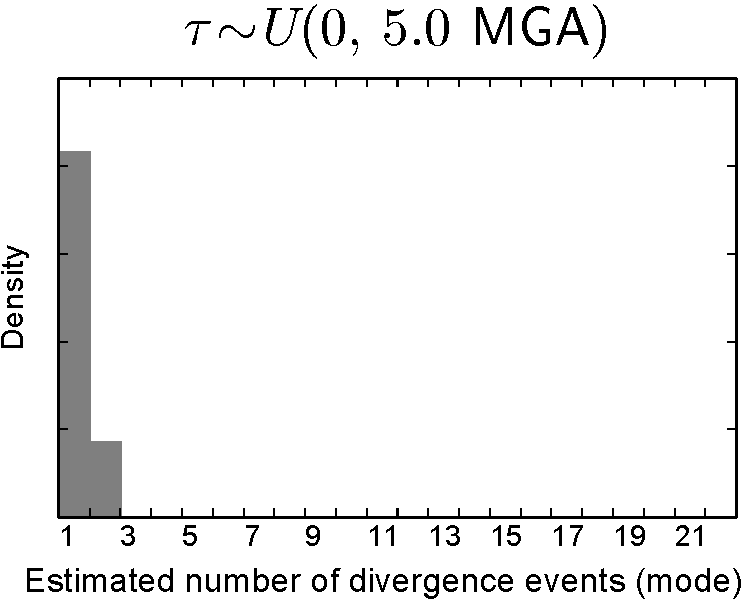
\includegraphics[width=0.5\textwidth]{../images/old_old_power_psi_mode_last.pdf}
        \end{center}
    \end{onlyenv}
    \begin{onlyenv}<2->
        \begin{block}{Objective:}
            Use principles of probability to extend \msb framework for improved
            estimation of shared evolutionary history
        \end{block}
    \end{onlyenv}
    \barefootnote{\tiny\shortfullcite{Oaks2012}. \hspace{2mm}\shortfullcite{Oaks2014reply}}
\end{frame}

\begin{frame}
    \frametitle{An improved method}
    Potential improvements:
    \begin{enumerate}
        \item Alternative priors on model parameters that improve marginal
            likelihoods of rich models
        \item Alternative prior over divergence models
        % \item Broad uniform priors on many of the model's parameters, including
        %     divergence times
        % \begin{itemize}
        %     \item Small marginal likelihoods of rich models
        % \end{itemize}
        % % \item Uniform priors on many of the model's parameters, including
        % %     divergence times
        % \item Prior on divergence models that, coupled with \#1, favors
        %     models with few divergence events
    \end{enumerate}
    \barefootnote{\tiny\shortfullcite{Oaks2012}. \hspace{2mm}\shortfullcite{Oaks2014reply}}
\end{frame}

\begin{frame}[t]
    \vspace{-2mm}
    \begin{displaybox}[5.5cm]
        \small
        \[
            p(X) = \int_{\theta} p(X \given \theta) p(\theta) \mathrm{d}\theta
        \]%\vspace{0mm}
    \end{displaybox}

    \vspace{-1mm}
    \begin{center}
        \includegraphics<1>[height=7.8cm]{../images/marginal-plot-2d-uniform-prior.pdf}
        \includegraphics<2>[height=7.8cm]{../images/marginal-plot-3d.png}
        \includegraphics<3>[height=7.8cm]{../images/marginal-plot-2d-uniform-prior.pdf}
        \includegraphics<4>[height=7.8cm]{../images/marginal-plot-2d.pdf}
    \end{center}
\end{frame}

\begin{frame}
    \frametitle{An improved method}
    Potential improvements:
    \begin{enumerate}
        \item Alternative priors on model parameters that improve marginal
            likelihoods of rich models
        \item Alternative prior over divergence models
    \end{enumerate}
    \barefootnote{\tiny\shortfullcite{Oaks2012}. \hspace{2mm}\shortfullcite{Oaks2014reply}}
\end{frame}

\begin{frame}
    \frametitle{Prior on divergence models}
    \begin{itemize}
        \item \msb uses a discrete uniform prior on the \emph{number} of
            divergence events
    \end{itemize}
    % \smallskip
    \centerline{
        \includegraphics<1->[width=\textwidth]{../images/partition_numbers.pdf}}
    \begin{block}<2->{\it Potential solution:}
        Place flexible prior directly on the sample space of divergence models
    \end{block}
\end{frame}


\begin{frame}
    \frametitle{New method: \dppmsbayes}
    \begin{itemize}
        % \item<1-> Reparameterized the model implemented in \msb
        \item<1-> Replaced uniform priors on continuous parameters with gamma and
            beta distributions
        \item<1-> Dirichlet process prior (DPP) over all possible divergence
            models
        % \item<4-> Uniform prior over divergence models
    \end{itemize}
\end{frame}

\begin{frame}
    \frametitle{\dppmsbayes: Simulation-based assessment}
        Simulate 50,000 datasets under three models\\
        \smallskip
        \begin{description}
            \item[$M_{msBayes}$]
                \begin{itemize}
                    \item U-shaped prior on divergence models
                    \item Uniform priors on continuous parameters
                \end{itemize}
            \smallskip
            \item[$M_{Ushaped}$]
                \begin{itemize}
                    \item U-shaped prior on divergence models
                    \item Gamma priors on continuous parameters
                \end{itemize}
            \smallskip
            % \item[$M_{Uniform}$]
            %     \begin{itemize}
            %         \item Uniform prior on divergence models
            %         \item Gamma priors on continuous parameters
            %     \end{itemize}
            % \smallskip
            \item[$M_{DPP}$]
                \begin{itemize}
                    \item DPP prior on divergence models
                    \item Gamma priors on continuous parameters
                \end{itemize}
        \end{description}
        \smallskip
        Analyze all datasets under each of the models
\end{frame}

\begin{frame}
    \frametitle{\dppmsbayes: Simulation results}
    \centerline{
        \includegraphics<1>[width=0.85\textwidth]{../images/validation-model-choice-old-dpp.pdf}
        \includegraphics<2>[width=1.13\textwidth]{../images/validation-model-choice-old-dpp-full.pdf}}
    \barefootnote{\shortfullcite{Oaks2014dpp}}
\end{frame}

\begin{frame}
    \frametitle{\dppmsbayes: Simulation-based power analyses}
    \begin{myitemize}
        \item Simulate datasets in which all 22 divergence times are random
        \uncover{
            \smallskip
            \begin{myitemize}
                \item $\divTime{} \sim U(0, \,0.5 \,MGA)$
                \smallskip
                \item $\divTime{} \sim U(0, \,1.5 \,MGA)$
                \smallskip
                \item $\divTime{} \sim U(0, \,2.5 \,MGA)$
                \smallskip
                \item $\divTime{} \sim U(0, \,5.0 \,MGA)$
                \smallskip
            \end{myitemize}
        \item $MGA$ = Millions of Generations Ago
        }
        \item Simulate 1000 datasets for each \divTime{} distribution
        % \item Analyze all 4000 datasets as we did the empirical data
        \item Analyze all 4000 datasets under models $M_{msBayes}$, $M_{Ushaped}$, and $M_{DPP}$
    \end{myitemize}
\end{frame}

\begin{frame}[t]
    \frametitle{\dppmsbayes: Power results}
    \vspace{1cm}
        \centerline{
        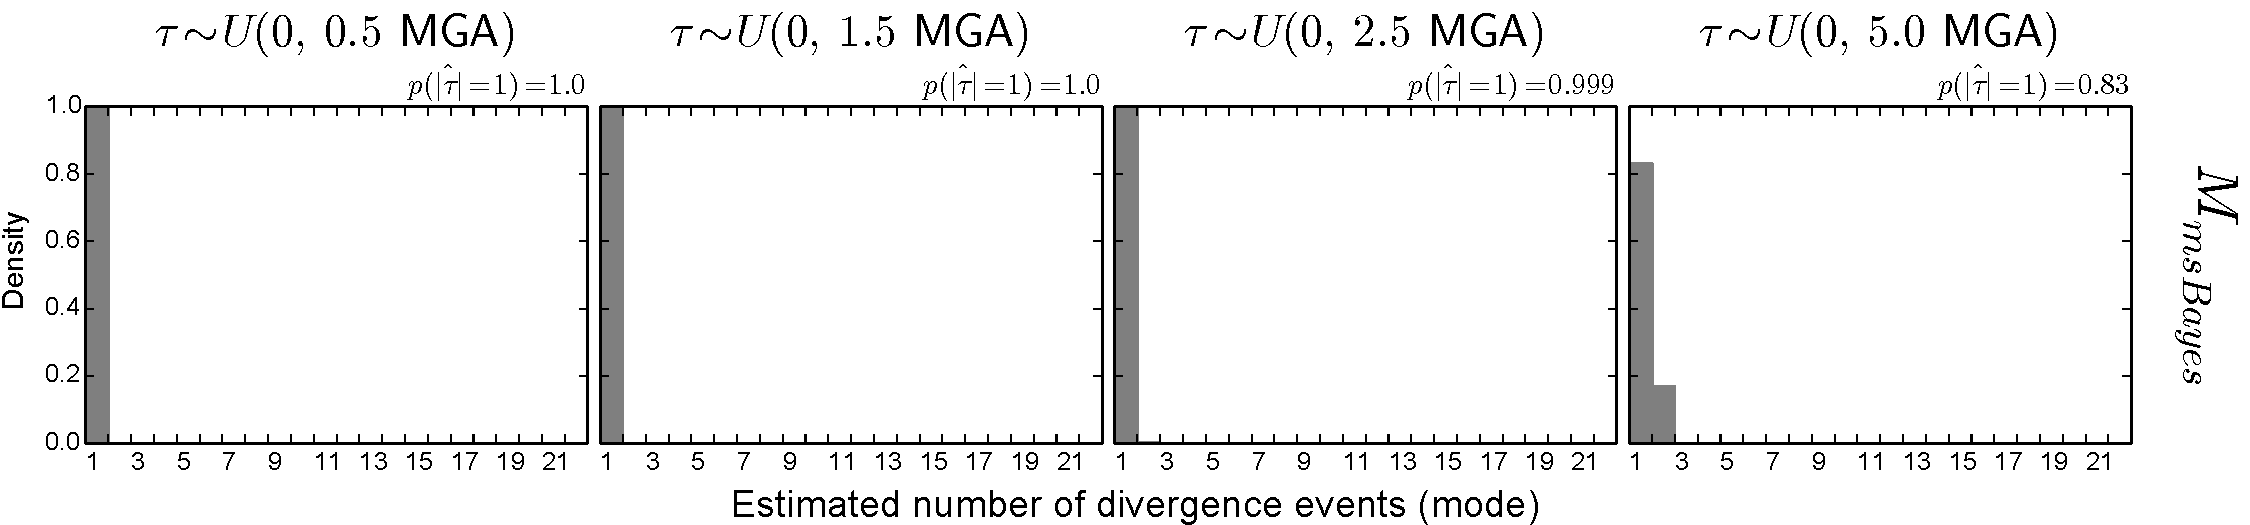
\includegraphics[width=1.13\textwidth]{../images/old_old_power_psi_mode.pdf}}
        \vspace{0mm}
        \centerline{
        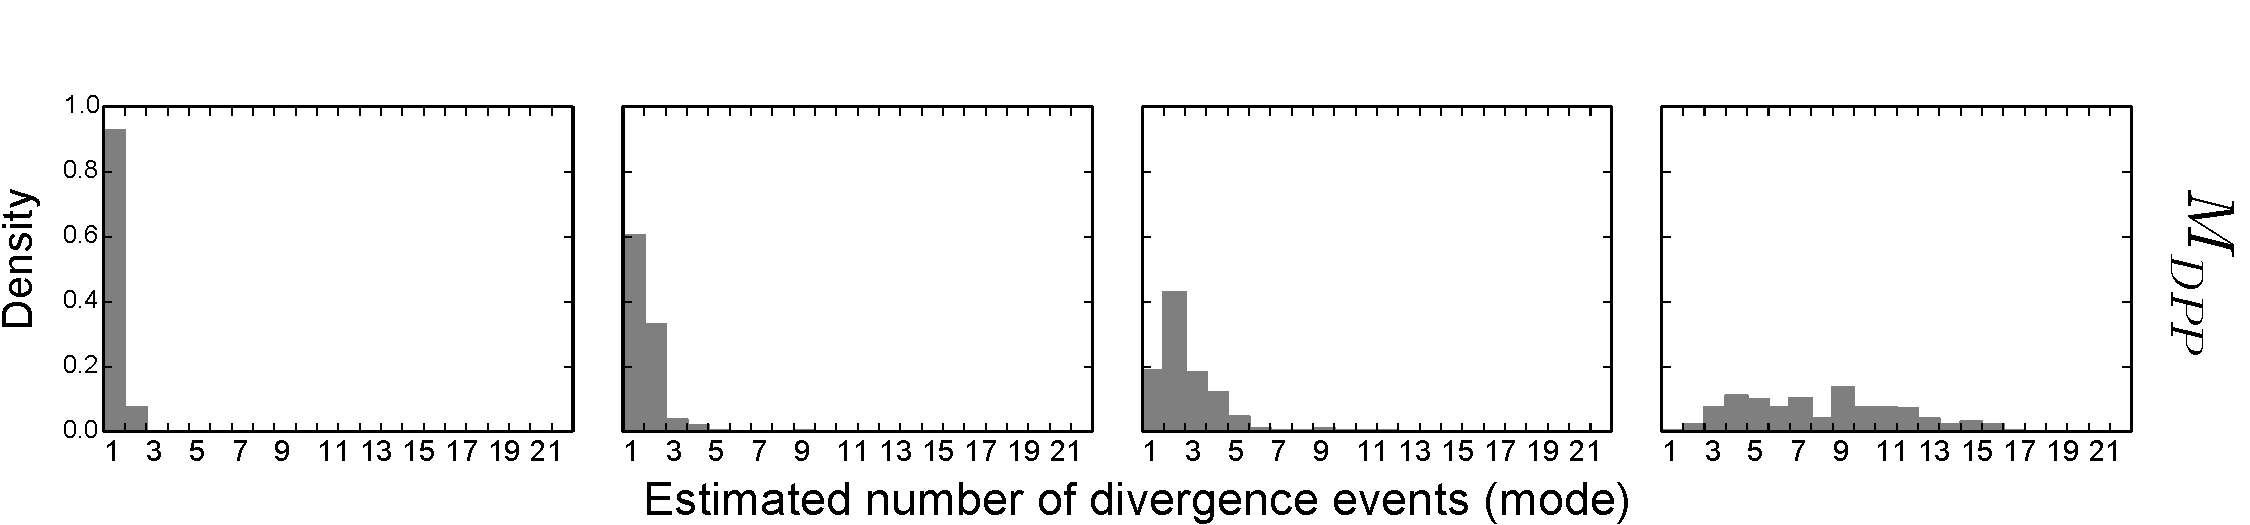
\includegraphics[width=1.13\textwidth]{../images/old_dpp_power_psi_mode_headless.pdf}}
    \barefootnote{\shortfullcite{Oaks2014dpp}}
\end{frame}

\begin{frame}[t]
    \frametitle{\dppmsbayes: Power results}
    \vspace{1cm}
        \centerline{
        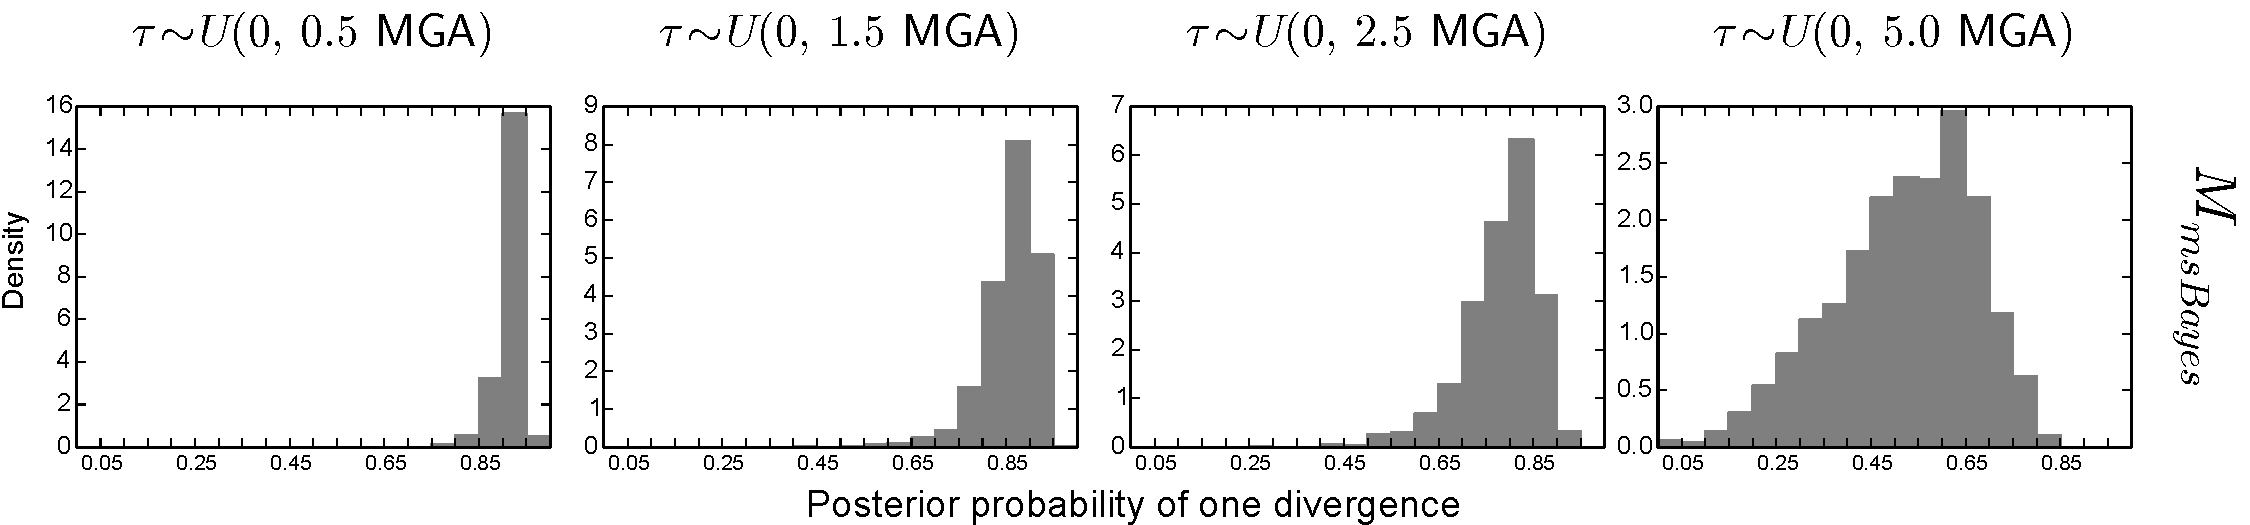
\includegraphics[width=1.13\textwidth]{../images/old_old_power_psi_prob.pdf}}
        \vspace{0mm}
        \centerline{
        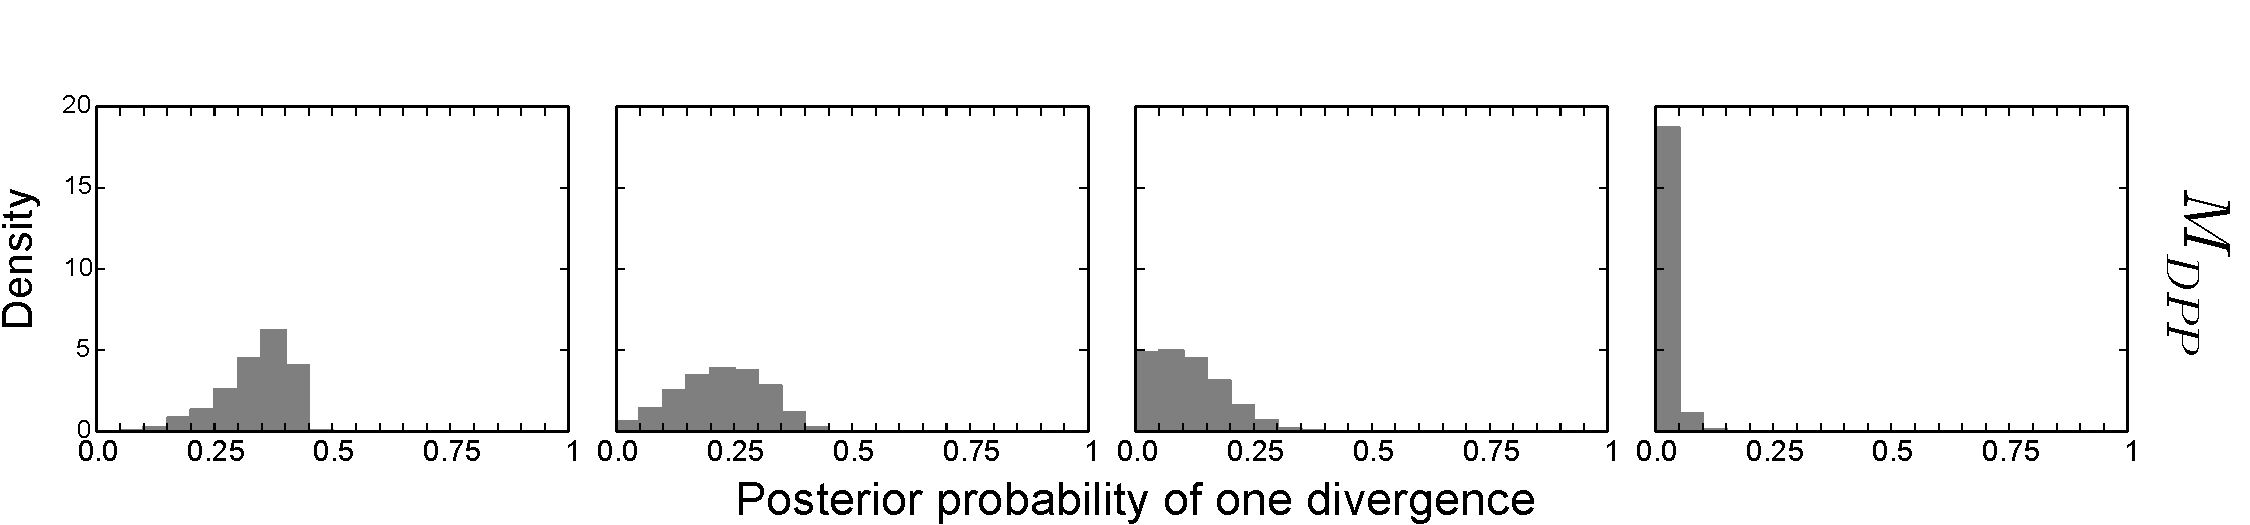
\includegraphics[width=1.13\textwidth]{../images/old_dpp_power_psi_prob_headless.pdf}}
    \barefootnote{\shortfullcite{Oaks2014dpp}}
\end{frame}

\begin{frame}
    \frametitle{\dppmsbayes: Power results}
    % \vspace{1cm}
        \centerline{
        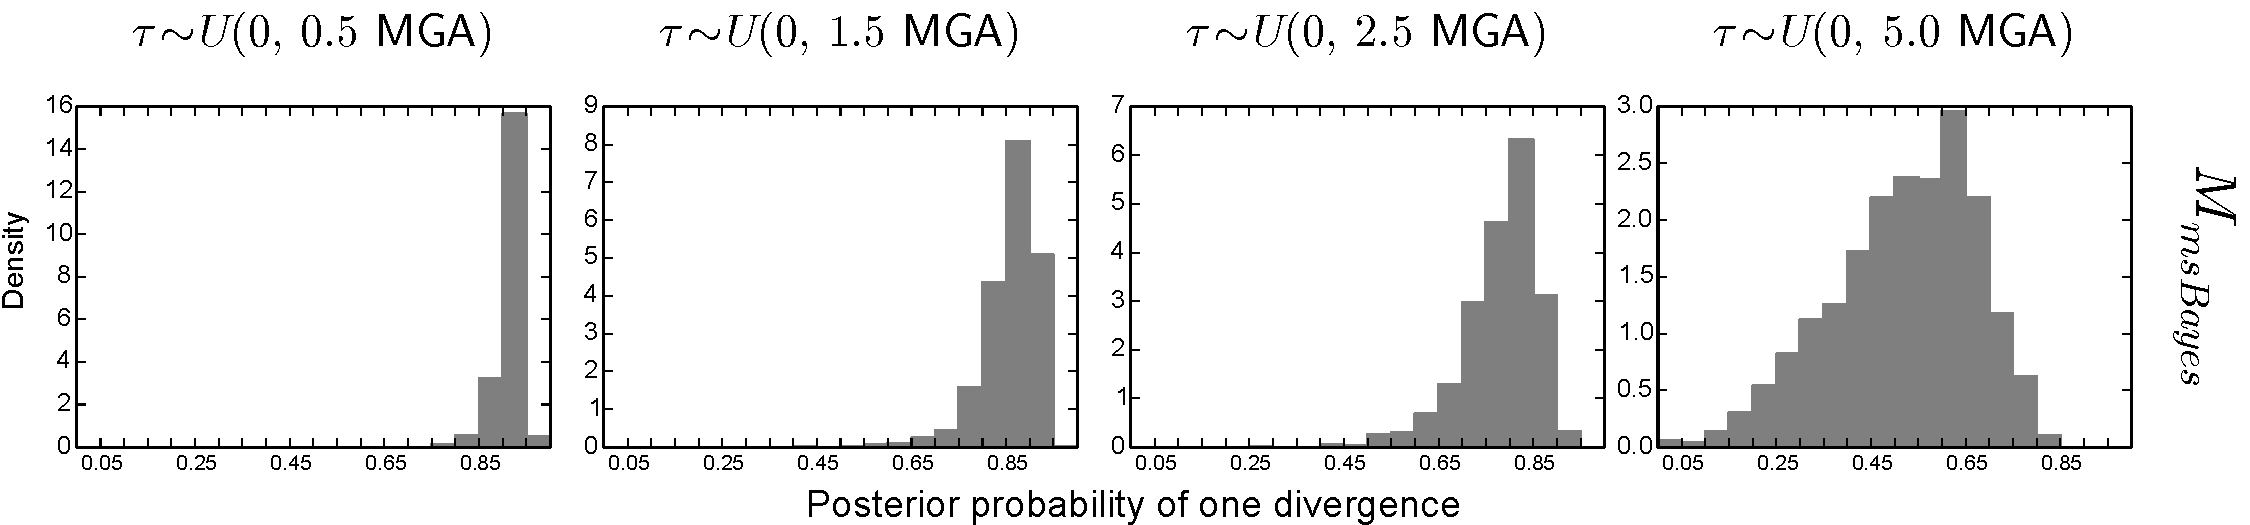
\includegraphics[width=\textwidth]{../images/old_old_power_psi_prob.pdf}}
        \vspace{0mm}
        \centerline{
        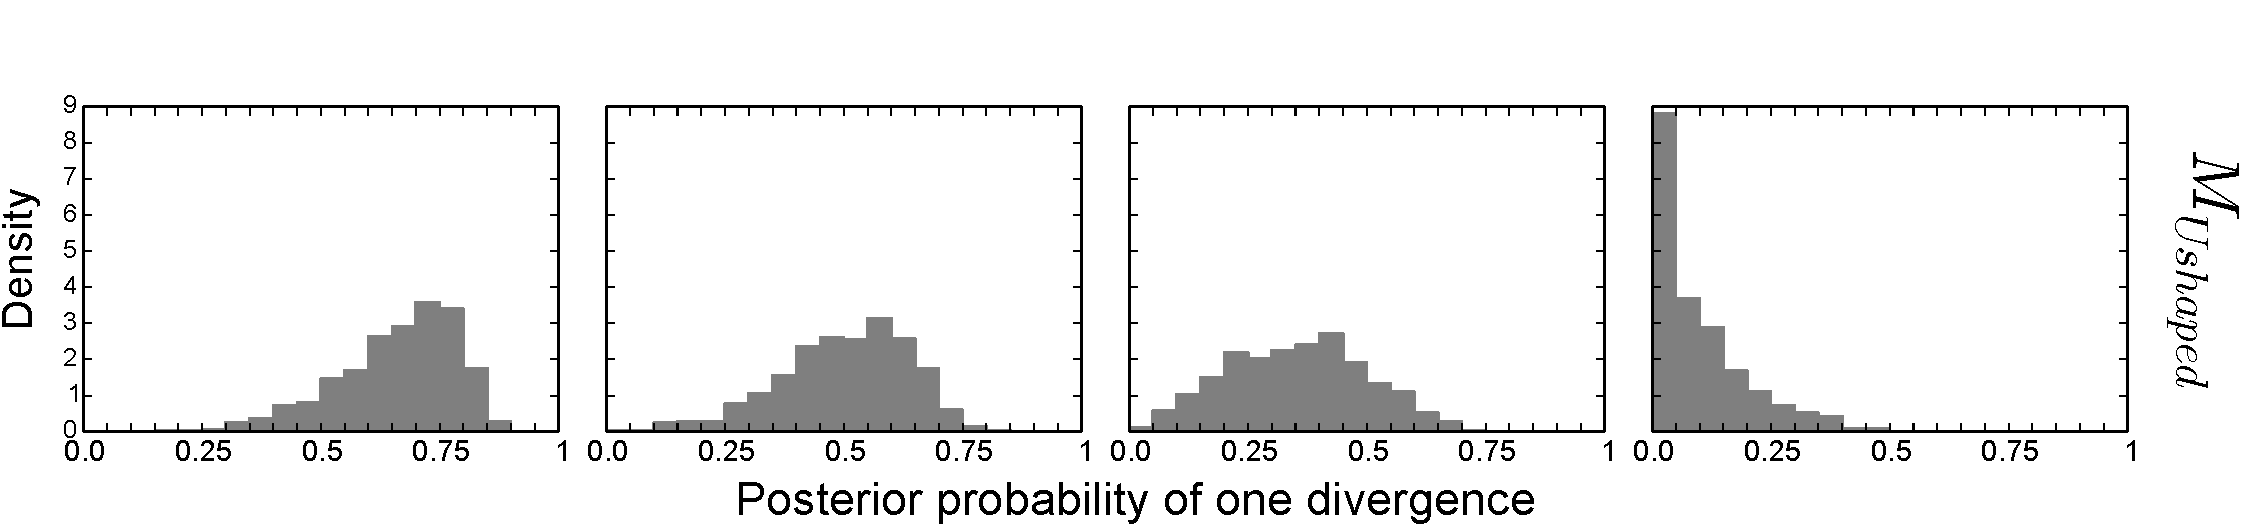
\includegraphics[width=\textwidth]{../images/old_u-shaped_power_psi_prob_headless.pdf}}
        \vspace{0mm}
        \centerline{
        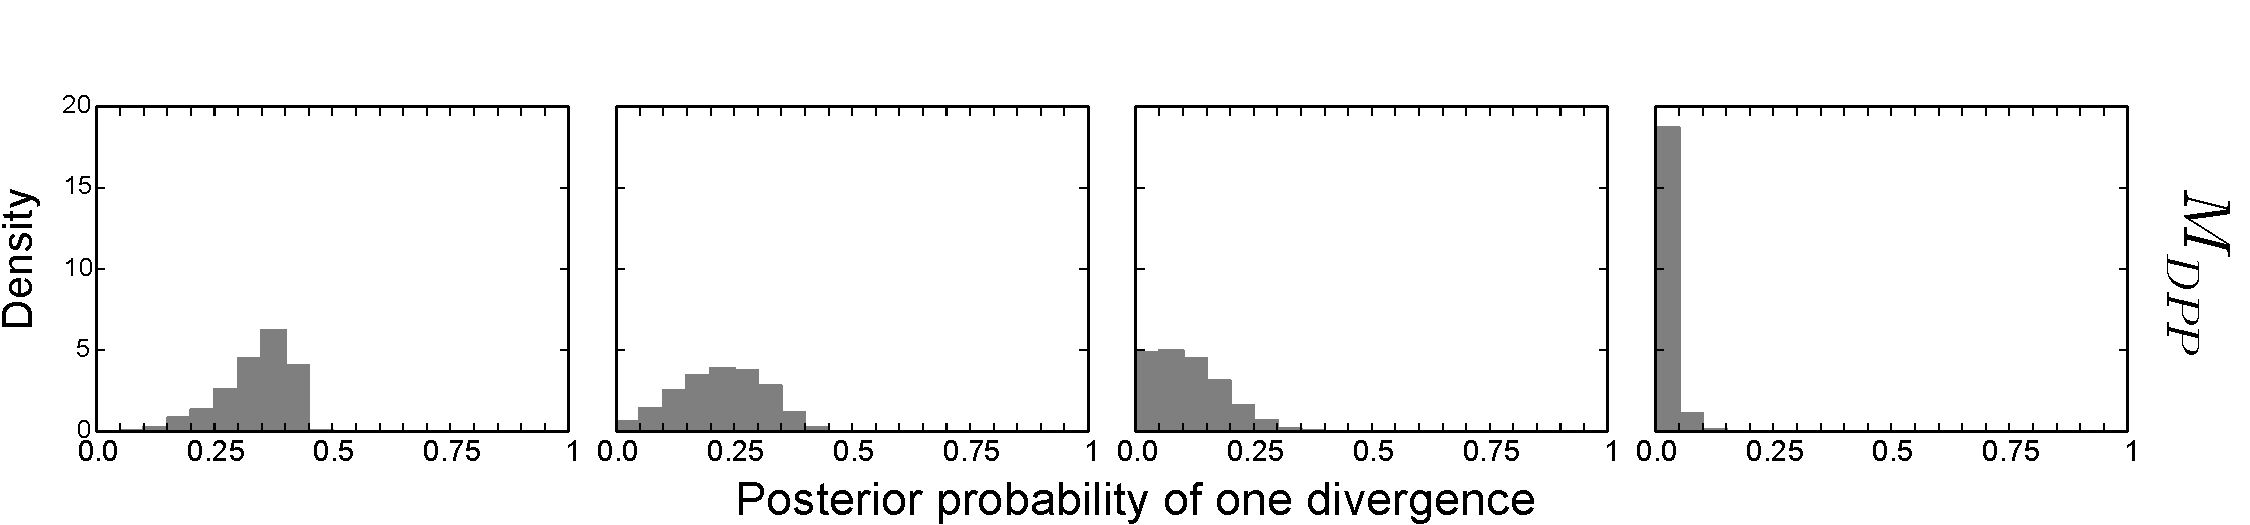
\includegraphics[width=\textwidth]{../images/old_dpp_power_psi_prob_headless.pdf}}
    % \barefootnote{\shortfullcite{Oaks2014dpp}}
\end{frame}

\begin{frame}
    \frametitle{Empirical application}
    \begin{columns}[c]
        \column{.5\textwidth}
        Did fragmentation of Philippine Islands during inter-glacial rises in
        sea level promote diversification?\\
        \begin{center}
            \includegraphics<1>[height=1.6cm]{../images/photos/gekko-mindorensis.jpg}
            \hspace{0.3mm}
            \includegraphics<1>[height=1.6cm]{../images/photos/sphenomorphus-arborens-rmb.jpg}

            \vspace{0.7mm}
            \includegraphics<1>[height=1.6cm]{../images/photos/dendrelaphis-pictus-cds.jpg}
            \hspace{0.3mm}
            \includegraphics<1>[height=1.6cm]{../images/photos/limnonectes-leytensis-rmb.jpg}

            \vspace{0.7mm}
            \includegraphics<1>[height=1.4cm]{../images/photos/hipposideros-obscurus-MRMDuya.jpg}
            \hspace{0.3mm}
            % \includegraphics<1>[height=1.2cm]{../images/photos/haplonycteris-fischeri-JHolden.jpg}
            % \hspace{0.1mm}
            \includegraphics<1>[height=1.4cm]{../images/photos/crocidura-negrina-JAEsselstyn.jpg}
        \end{center}
        \column{.5\textwidth}
        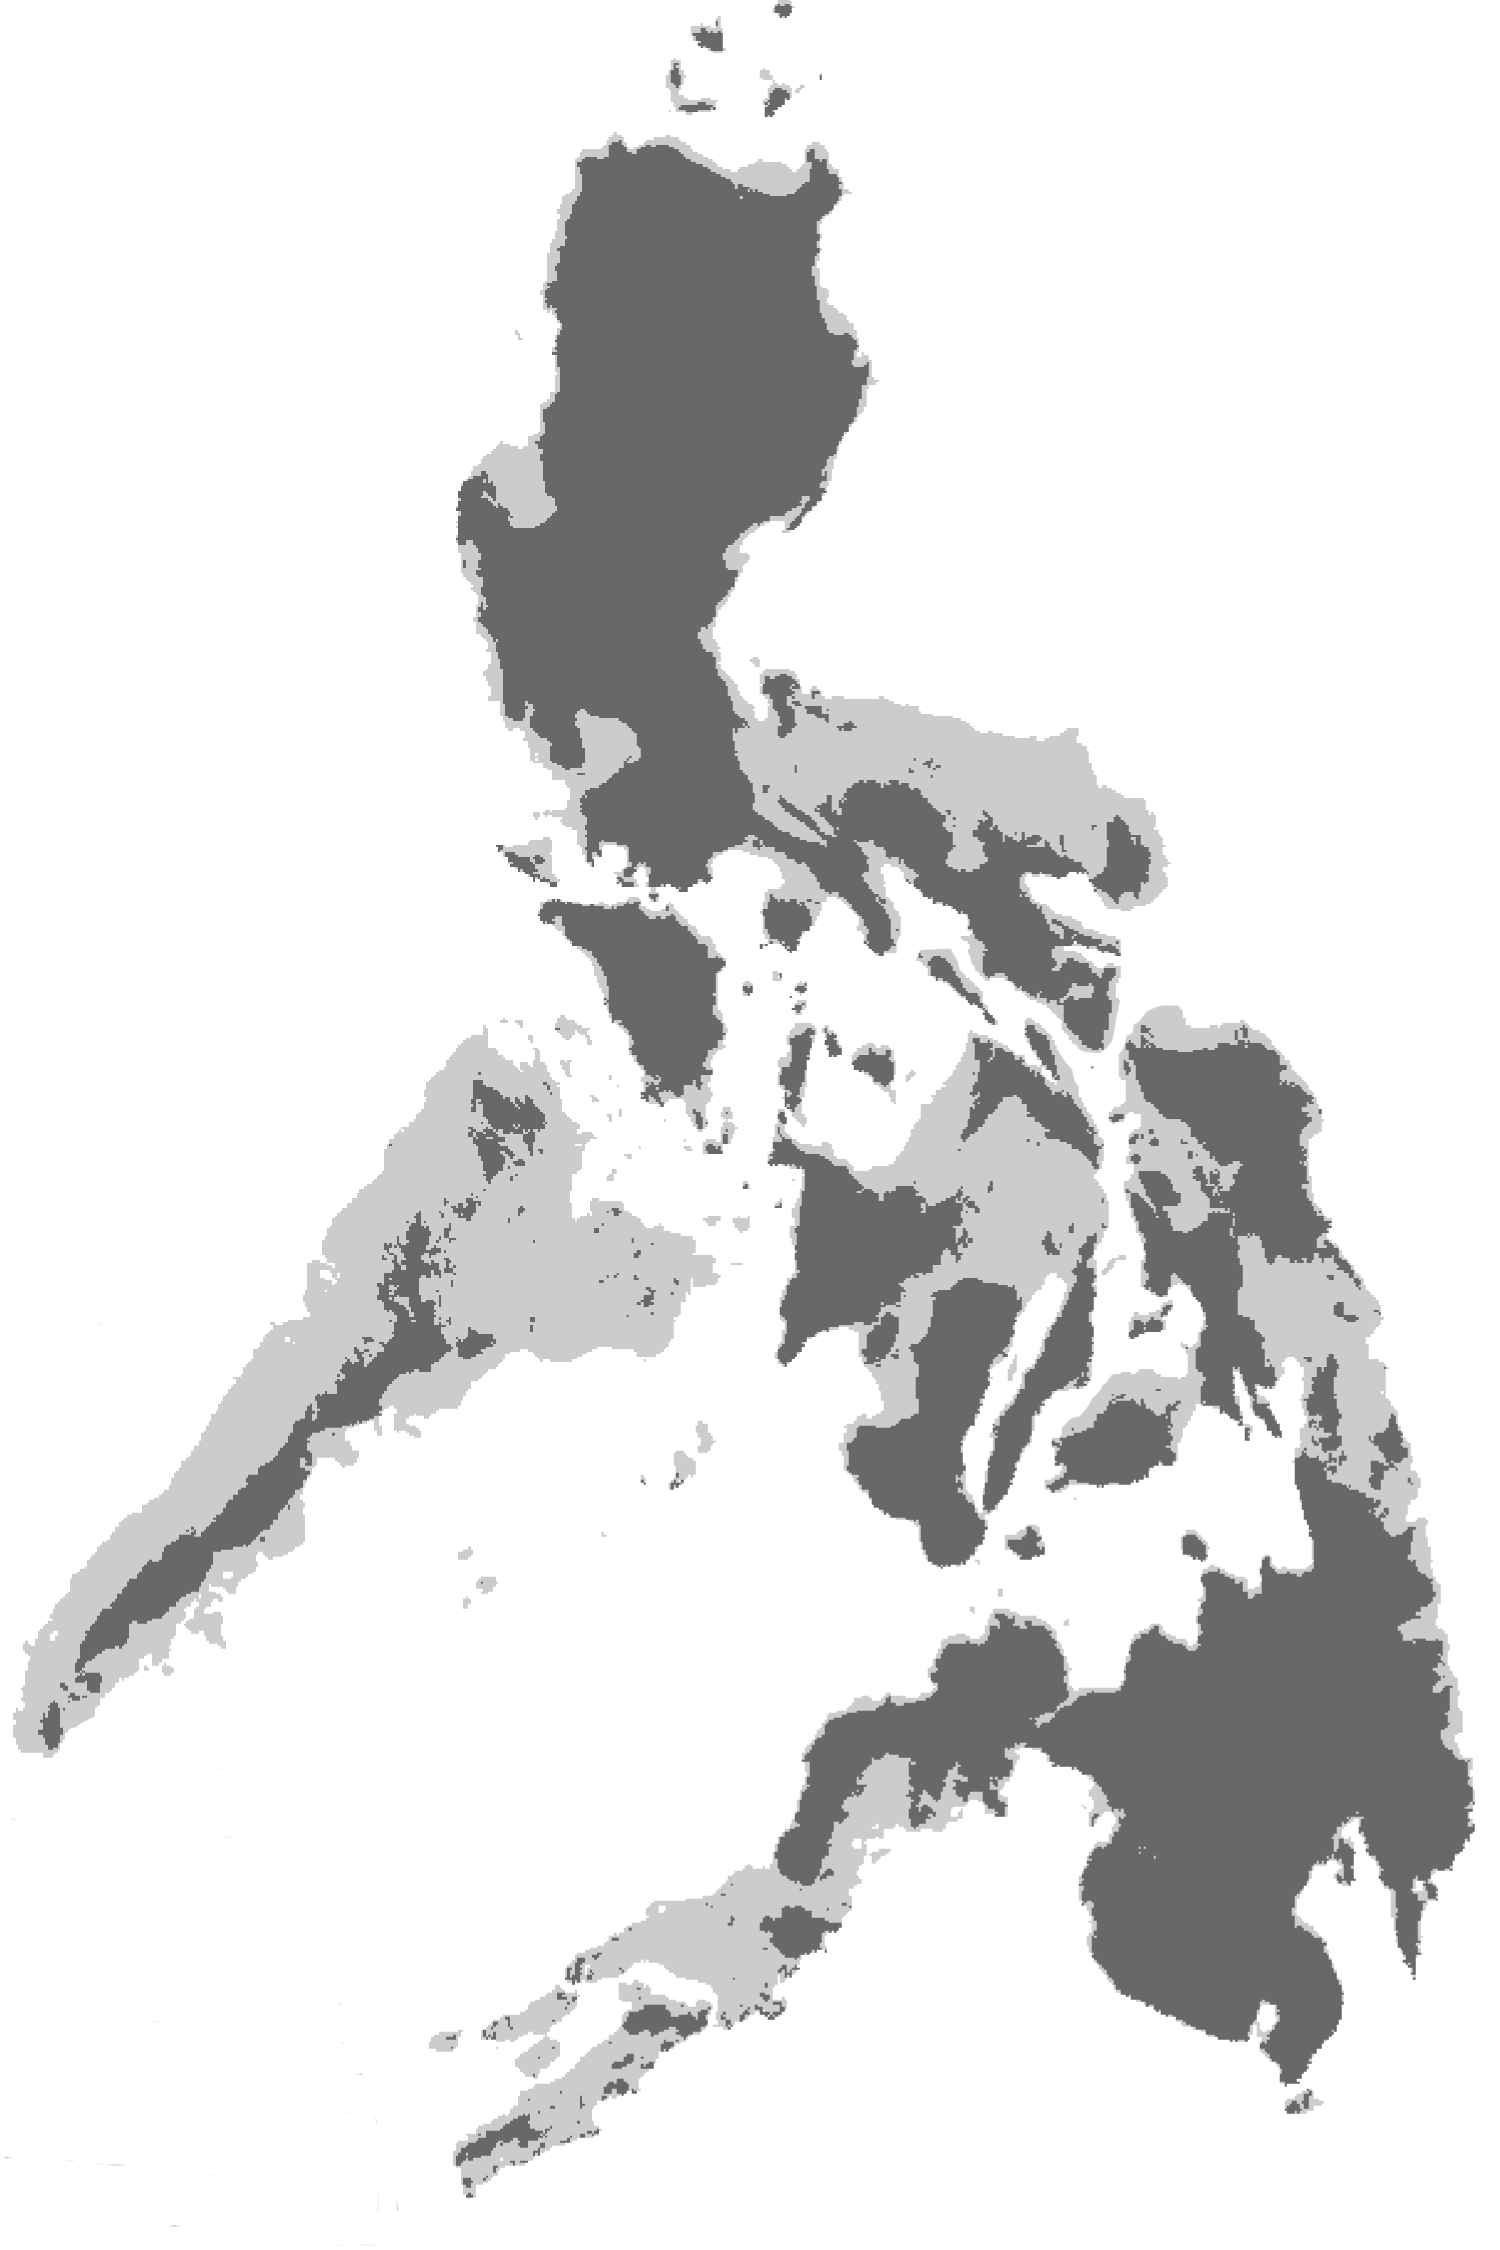
\includegraphics[width=\textwidth]{../images/maps/Philippines.png}
    \end{columns}
\end{frame}

\begin{frame}
    \frametitle{Empirical results: Philippine diversification}
    \centerline{
    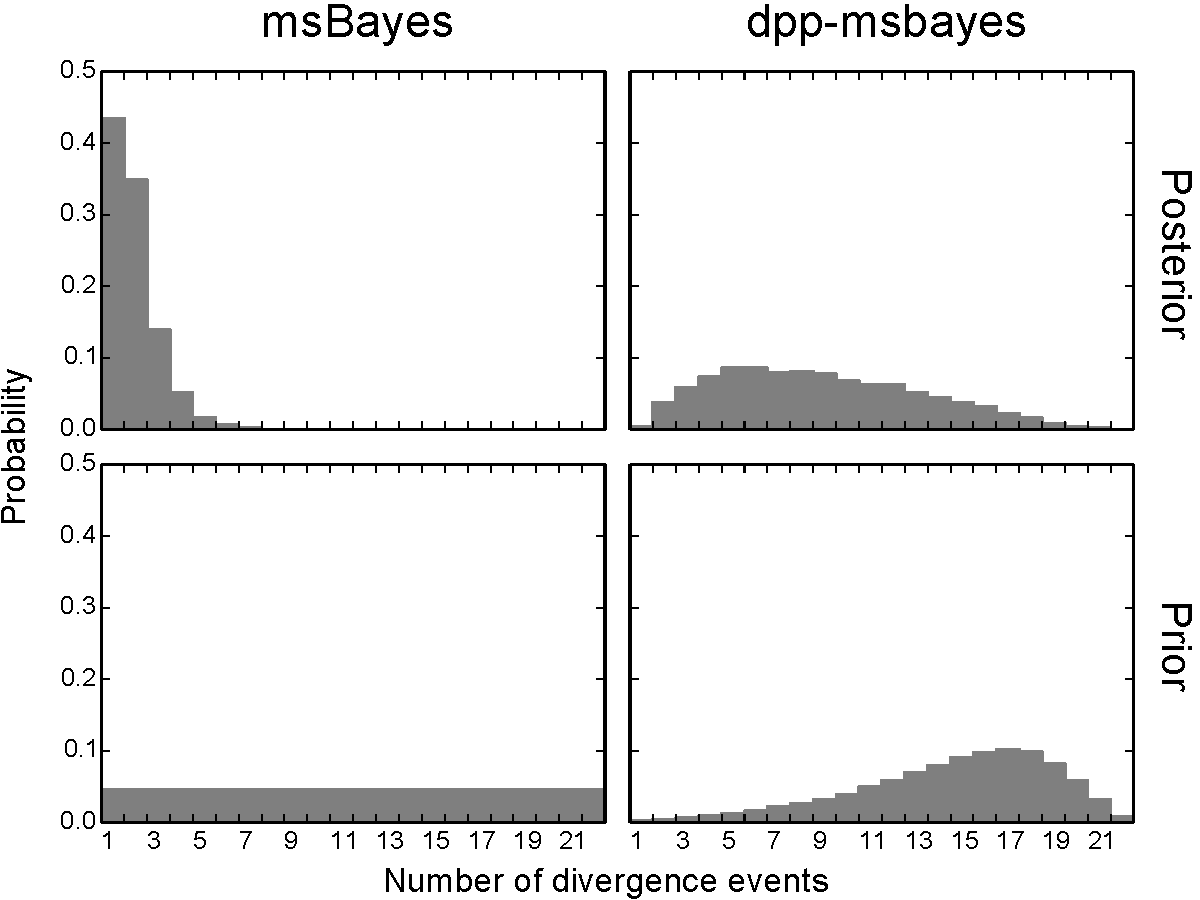
\includegraphics[width=0.8\textwidth]{../../empirical-analyses/plots/philippines-dpp-psi-posterior-old-vs-dpp-with-prior.pdf}}
    \barefootnote{\shortfullcite{Oaks2014dpp}}
\end{frame}

\section{Conclusions}

\begin{frame}
    \frametitle{Conclusions}
    \begin{itemize}
        \item<1-> New method for estimating shared evolutionary history shows
            improved
        \begin{enumerate}
            \item Estimates of posterior uncertainty
            \item Model-choice accuracy
            \item Power to detect temporal variation across divergences
            \item Robustness to model violations
        \end{enumerate}

        \item<2-> Improvement is due to
        \begin{enumerate}
            \item Alternative priors on model parameters avoid prohibitively
                small marginal likelihoods for models with more divergence
                events
            \item Nonparametric prior on the temporal distribution of
                divergences avoids combinatorial ``interaction'' with
                divergence-time priors
        \end{enumerate}
    \end{itemize}
\end{frame}

\begin{frame}
    \frametitle{Caveats}
    \begin{itemize}
        \item<1-> Estimating a very rich (600+ parameters for 22 taxa) model
            using limited information from the data

        \begin{itemize}
            \item Likely sensitive to prior assumptions
            \item Be skeptical of strongly supported results
        \end{itemize}

        \item<2-> ABC can be inaccurate for model choice
            \footnote{\tiny\shortfullcite{Robert2011}}
    \end{itemize}
\end{frame}

\begin{frame}
    \frametitle{Recommendations}
    For Bayesian model choice, choose priors carefully\\
    \bigskip
    ABC model choice estimates should be accompanied by:
    \begin{enumerate}
        \item Simulation-based power analyses
        \item Assessment of prior sensitivity
    \end{enumerate}
\end{frame}

\begin{frame}[t]
    \frametitle{Future directions}
    \begin{itemize}
        \item<1-> Full-likelihood Bayesian approach \footnote{\tiny\shortfullcite{JeetDiss}}
        \item<2-> Full-phylogenetic framework
    \end{itemize}
    
    \begin{center}
        \includegraphics<2>[height=5.5cm]{../images/div-model-cartoon-sp-tree-shared-wide.pdf}
        \includegraphics<3>[height=5.5cm]{../images/div-model-cartoon-sp-phylogeny.pdf}
    \end{center}
\end{frame}

\begin{frame}
    \frametitle{Software}
    Everything is on GitHub\ldots\\
    \smallskip
    \begin{itemize}
        \item \texttt{dpp-msbayes}:
            \href{https://github.com/joaks1/dpp-msbayes}{\tt
            https://github.com/joaks1/dpp-msbayes}

        \item \texttt{PyMsBayes}:
            \href{https://github.com/joaks1/PyMsBayes}{\tt
            https://github.com/joaks1/PyMsBayes}

        \item ABACUS: Approximate BAyesian C UtilitieS.
            \href{https://github.com/joaks1/abacus}{\tt
            https://github.com/joaks1/abacus}
    \end{itemize}
\end{frame}

\begin{frame}
    \frametitle{Open Notebook Science}
    Everything is on GitHub\ldots\\
    \smallskip
    \begin{itemize}
        \item \texttt{msbayes-experiments}:
            \href{https://github.com/joaks1/msbayes-experiments}{\tt
            https://github.com/joaks1/msbayes-experiments}
        % \item joaks1@gmail.com
    \end{itemize}
\end{frame}

\begin{frame}
    \frametitle{Acknowledgments}
    \begin{columns}[t]
        \column{.5\textwidth}
            {\bf Ideas and feedback:}
            \begin{myitemize}
                \item Holder Lab
                \item KU Herpetology
                \item Melissa Callahan
            \end{myitemize}
            \smallskip
            {\bf Computation:}
            \begin{myitemize}
                \item KU ITTC
                \item KU Computing Center
                \item iPlant
            \end{myitemize}
        \column{.5\textwidth}
            {\bf Funding:}
            \begin{myitemize}
                \item NSF
                \item KU Grad Studies, EEB \& BI
                \item SSB
                \item Sigma Xi
            \end{myitemize}
            \smallskip
            {\bf Photo credits:}
            \begin{myitemize}
                \item Rafe Brown, Cam Siler, \& Jake Esselstyn
                \item FMNH Philippine Mammal Website:
                    \begin{myitemize}
                        \item D.S.\ Balete, M.R.M.\ Duya, \& J.\ Holden
                    \end{myitemize}
            \end{myitemize}
    \end{columns}
\end{frame}

{
\usebackgroundtemplate{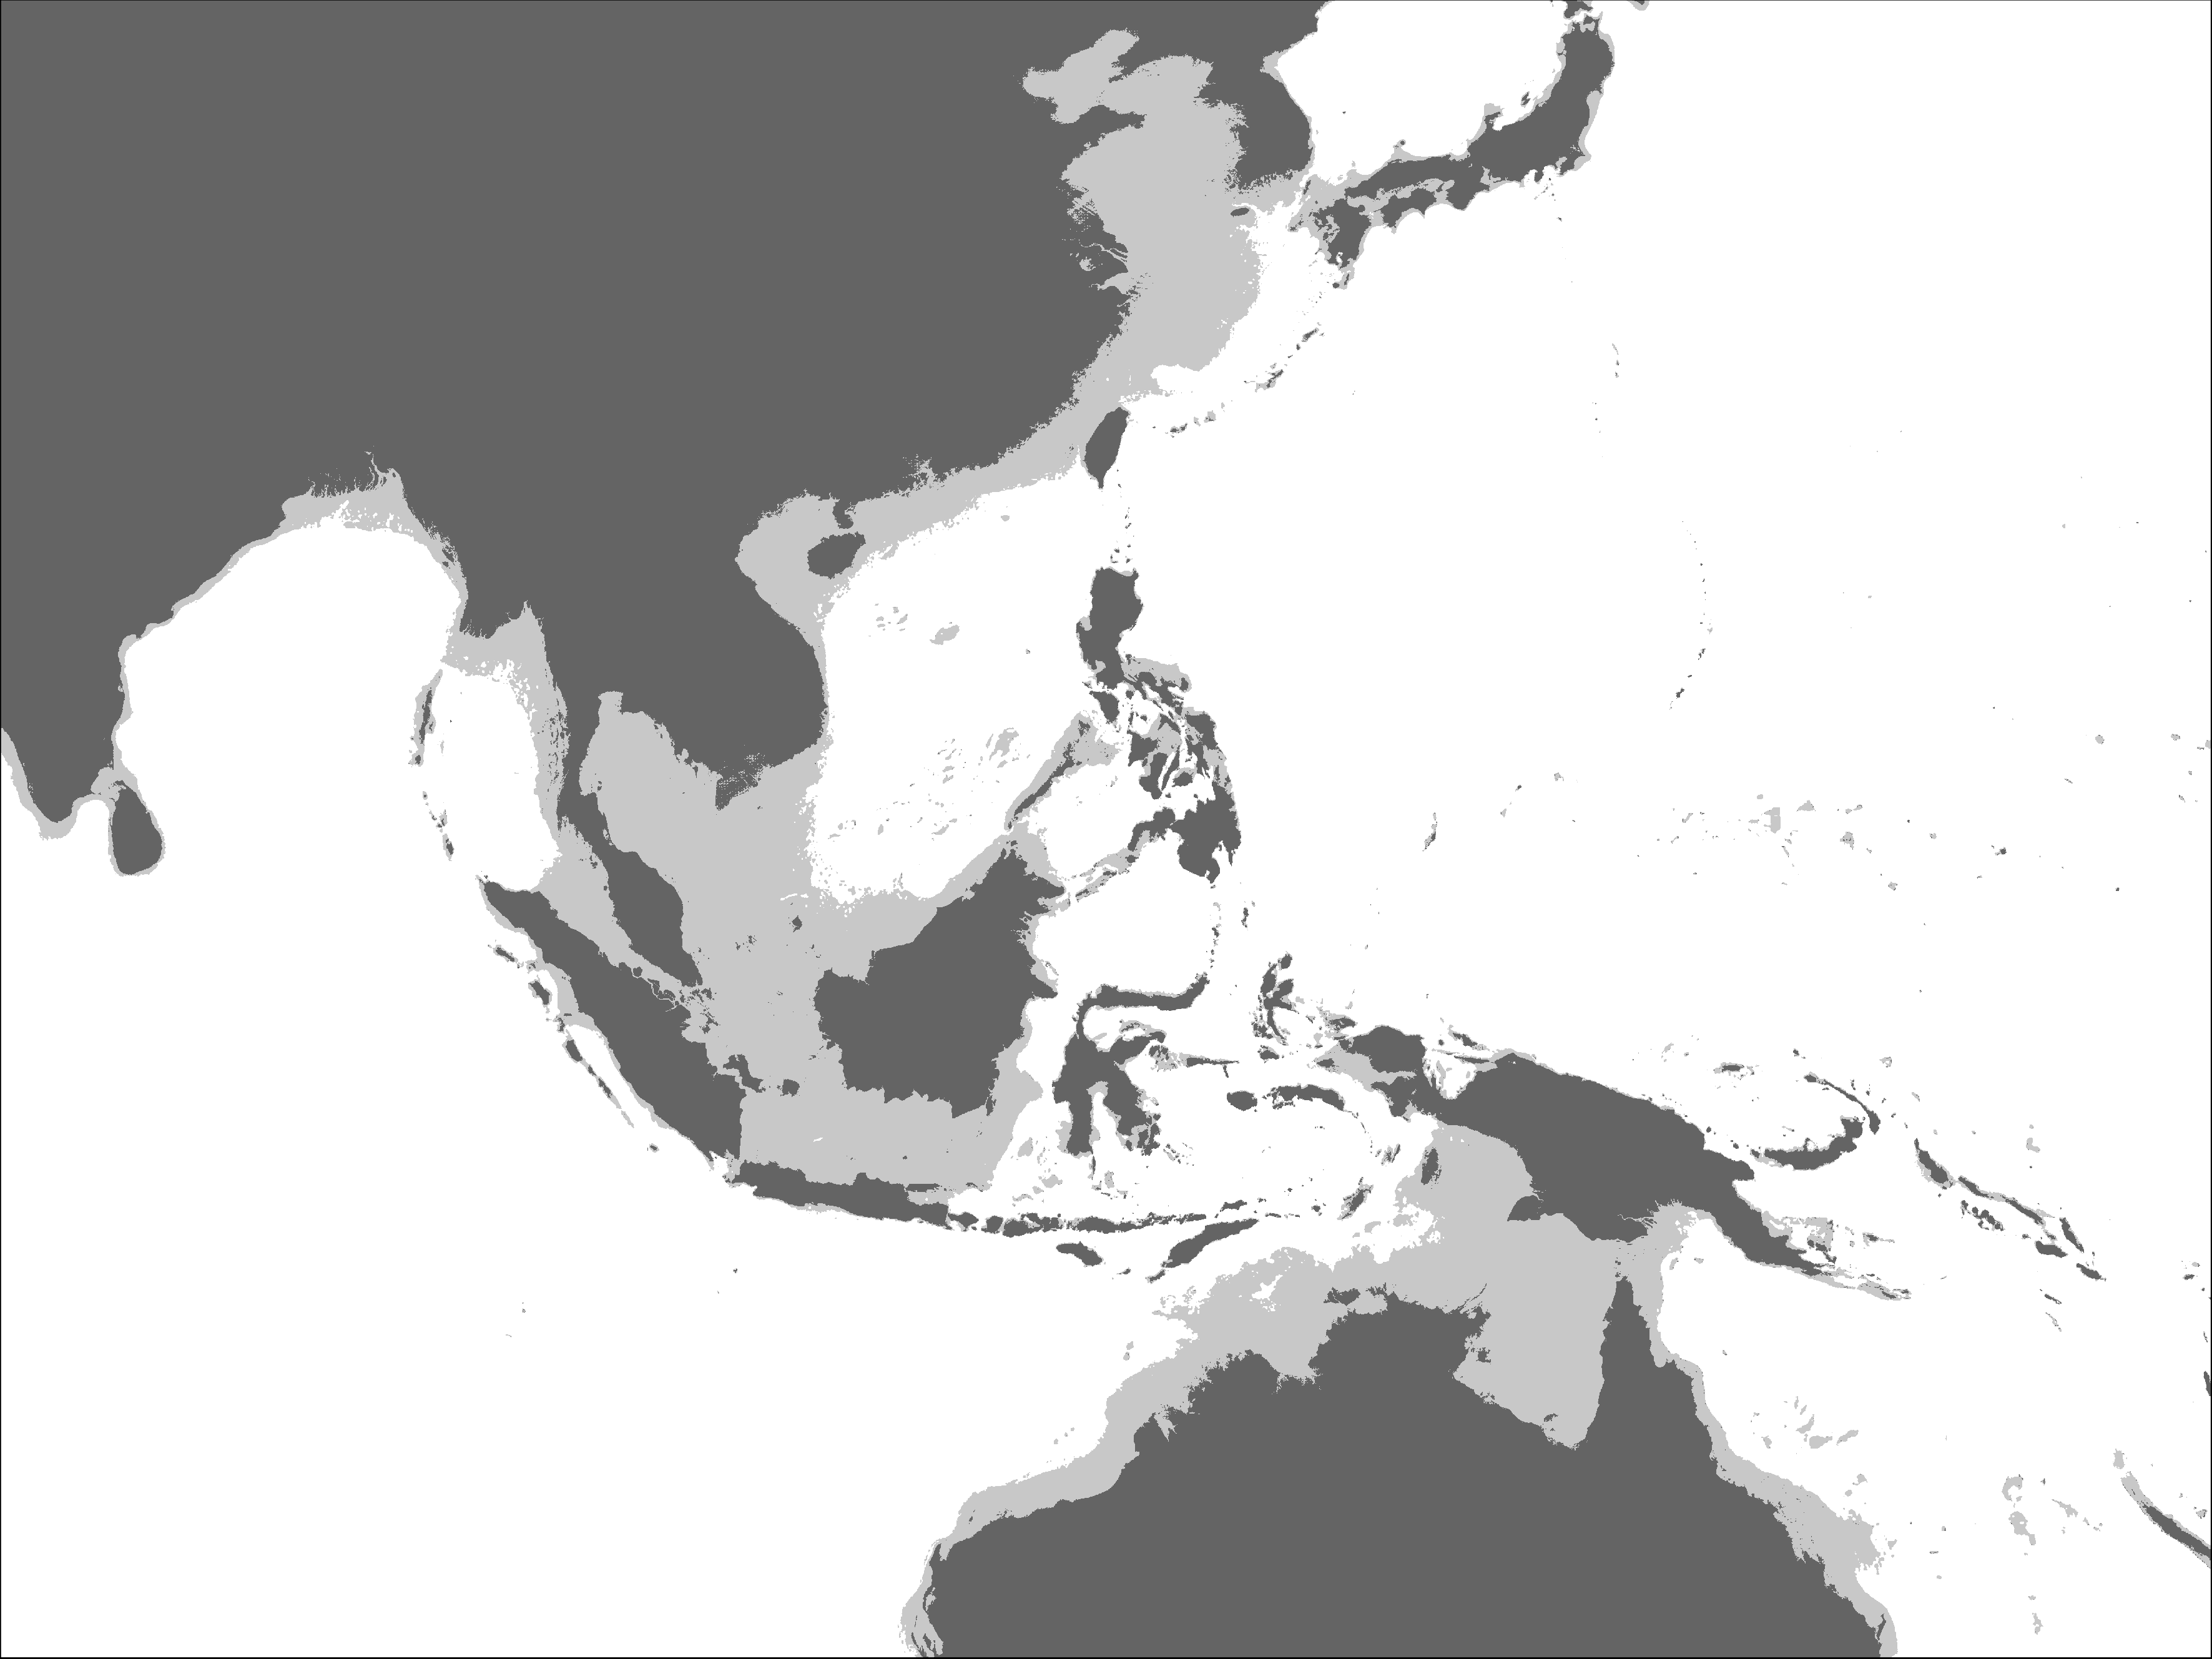
\includegraphics[width=\paperwidth]{../images/maps/se-asia-120.png}}
\begin{frame}
    \frametitle{Questions?}    
\end{frame}
}

% Extra slides

\begin{frame}[noframenumbering]
    \frametitle{Causes of bias: Insufficient sampling}
    \begin{itemize}
        \item Models with more parameter space are less densely sampled
        \item Could explain bias toward small models in extreme cases
        \item {\bf Predicts large variance in posterior estimates}
        \begin{itemize}
            \item We explored empirical and simulation-based analyses with
                2, 5, and 10 million prior samples, and estimates were
                very similar
        \end{itemize}
    \end{itemize}
    \smallskip
    \centerline{
    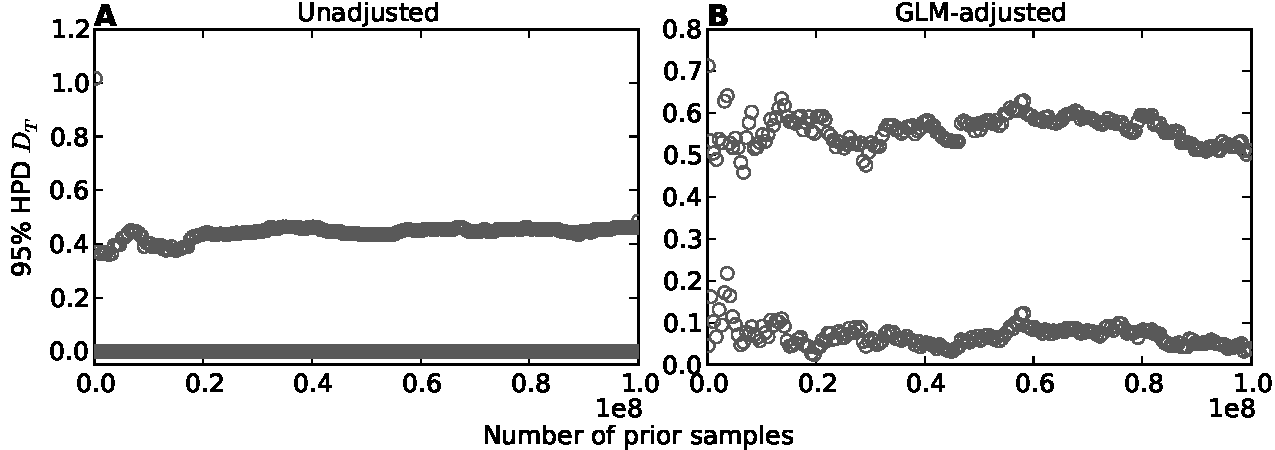
\includegraphics[width=\textwidth]{../images/omega_over_sampling.pdf}}
\end{frame}

\begin{frame}[noframenumbering]
    \frametitle{\dppmsbayes: Simulation results}
    % \vspace{1cm}
        \centerline{
        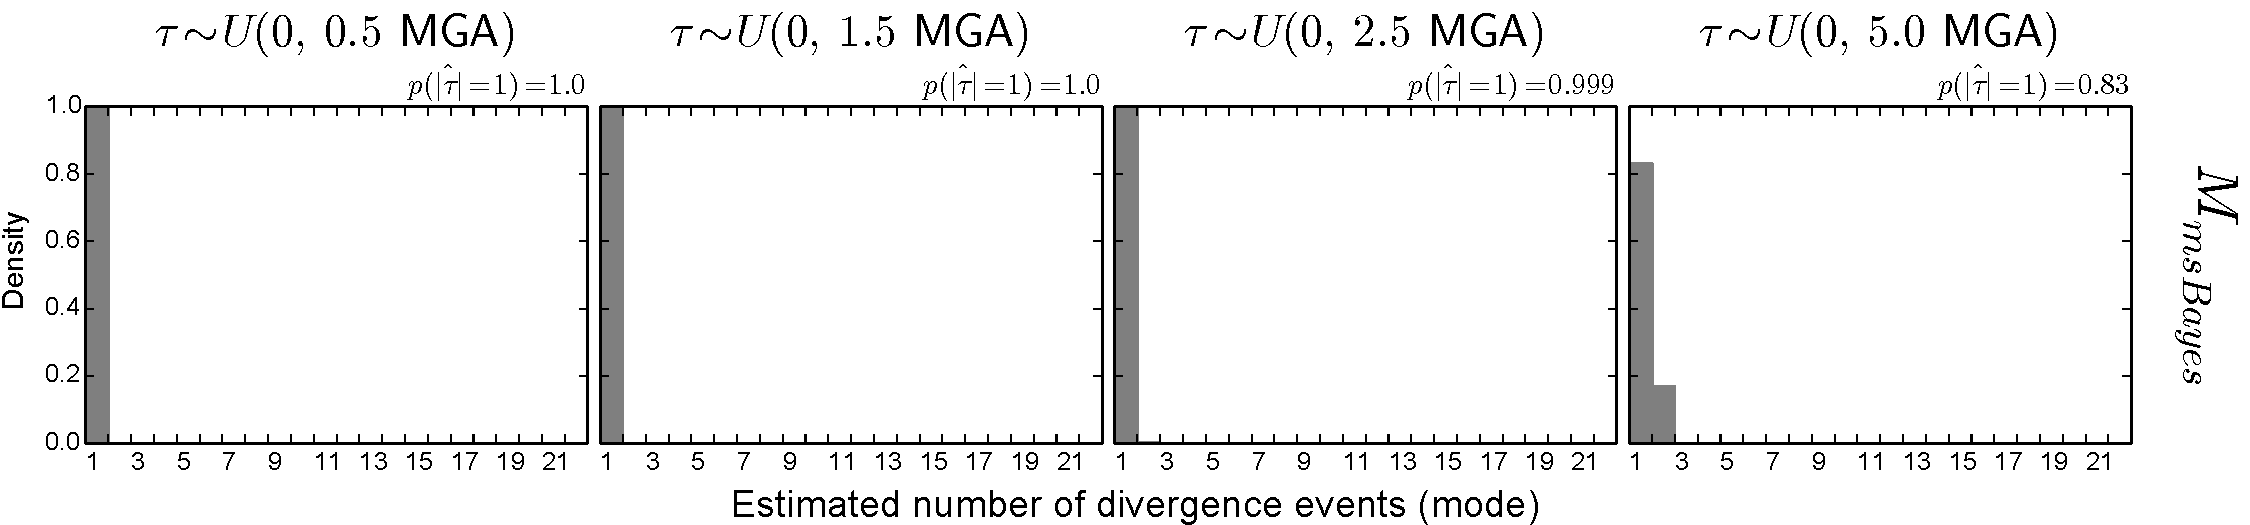
\includegraphics[width=\textwidth]{../images/old_old_power_psi_mode.pdf}}
        \vspace{0mm}
        \centerline{
        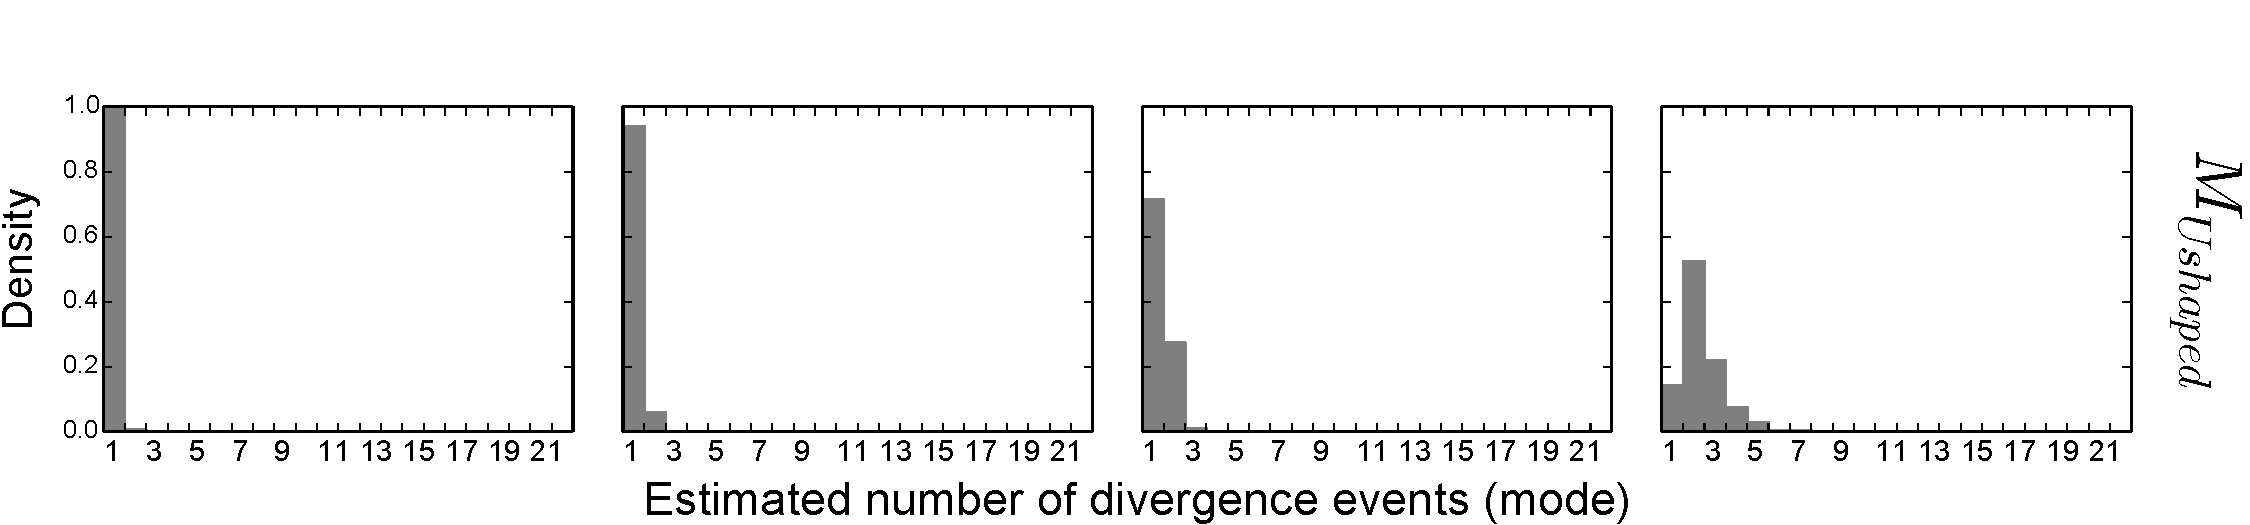
\includegraphics[width=\textwidth]{../images/old_u-shaped_power_psi_mode_headless.pdf}}
        \vspace{0mm}
        \centerline{
        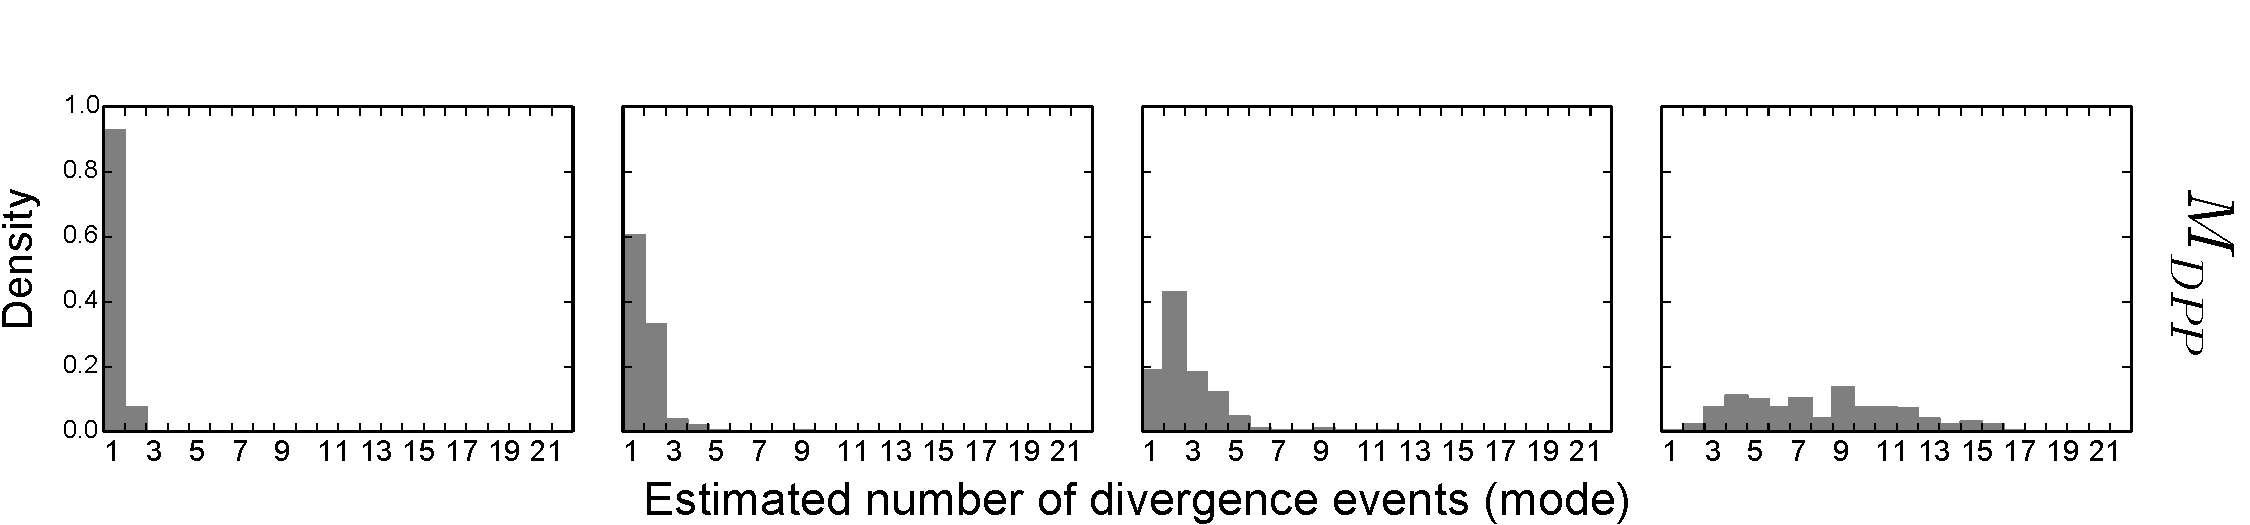
\includegraphics[width=\textwidth]{../images/old_dpp_power_psi_mode_headless.pdf}}
    % \barefootnote{\shortfullcite{Oaks2014dpp}}
\end{frame}

\begin{frame}[noframenumbering]
    \frametitle{\dppmsbayes: Simulation results}
    % \vspace{1cm}
        \centerline{
        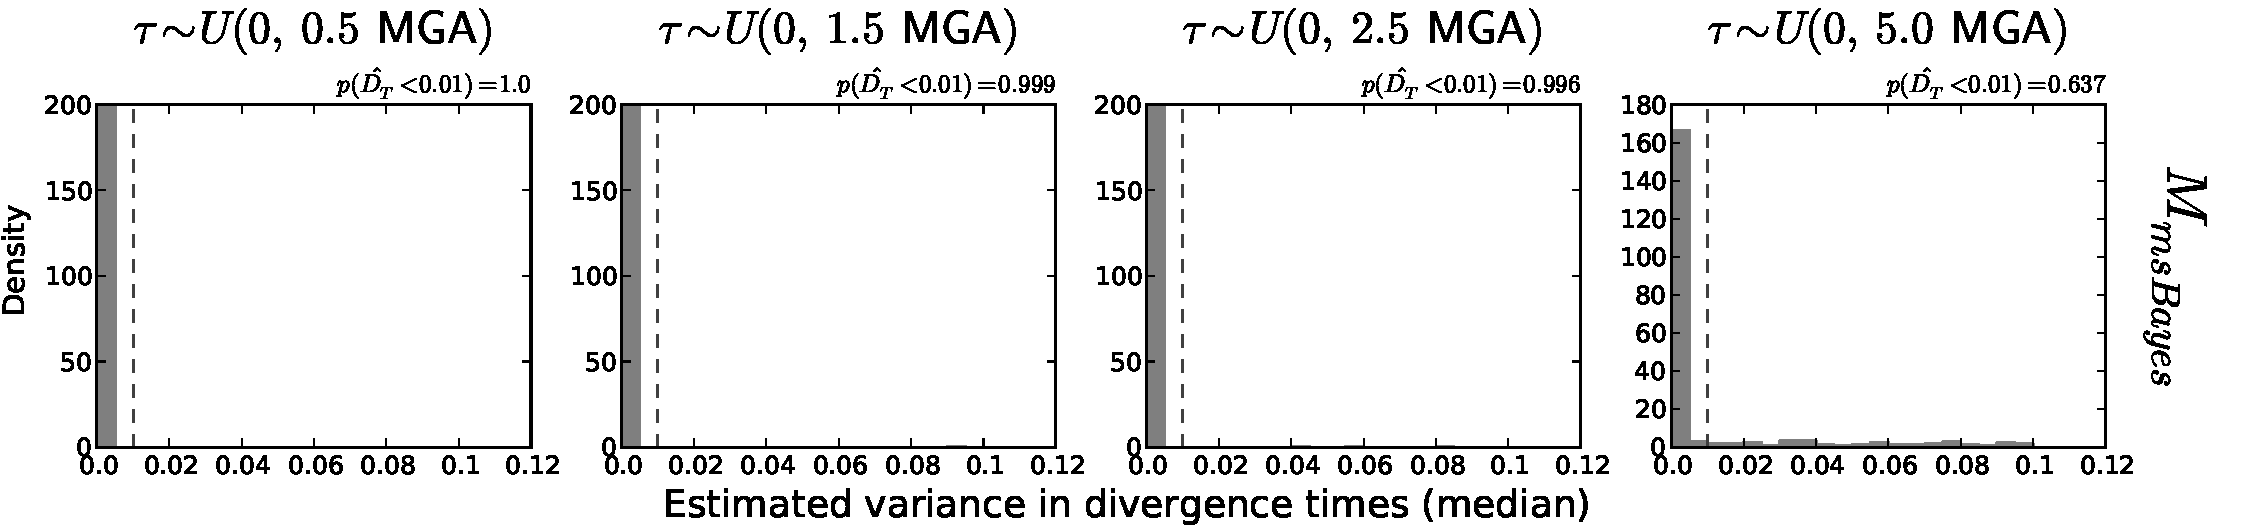
\includegraphics[width=\textwidth]{../images/old_old_power_omega_median.pdf}}
        \vspace{0mm}
        \centerline{
        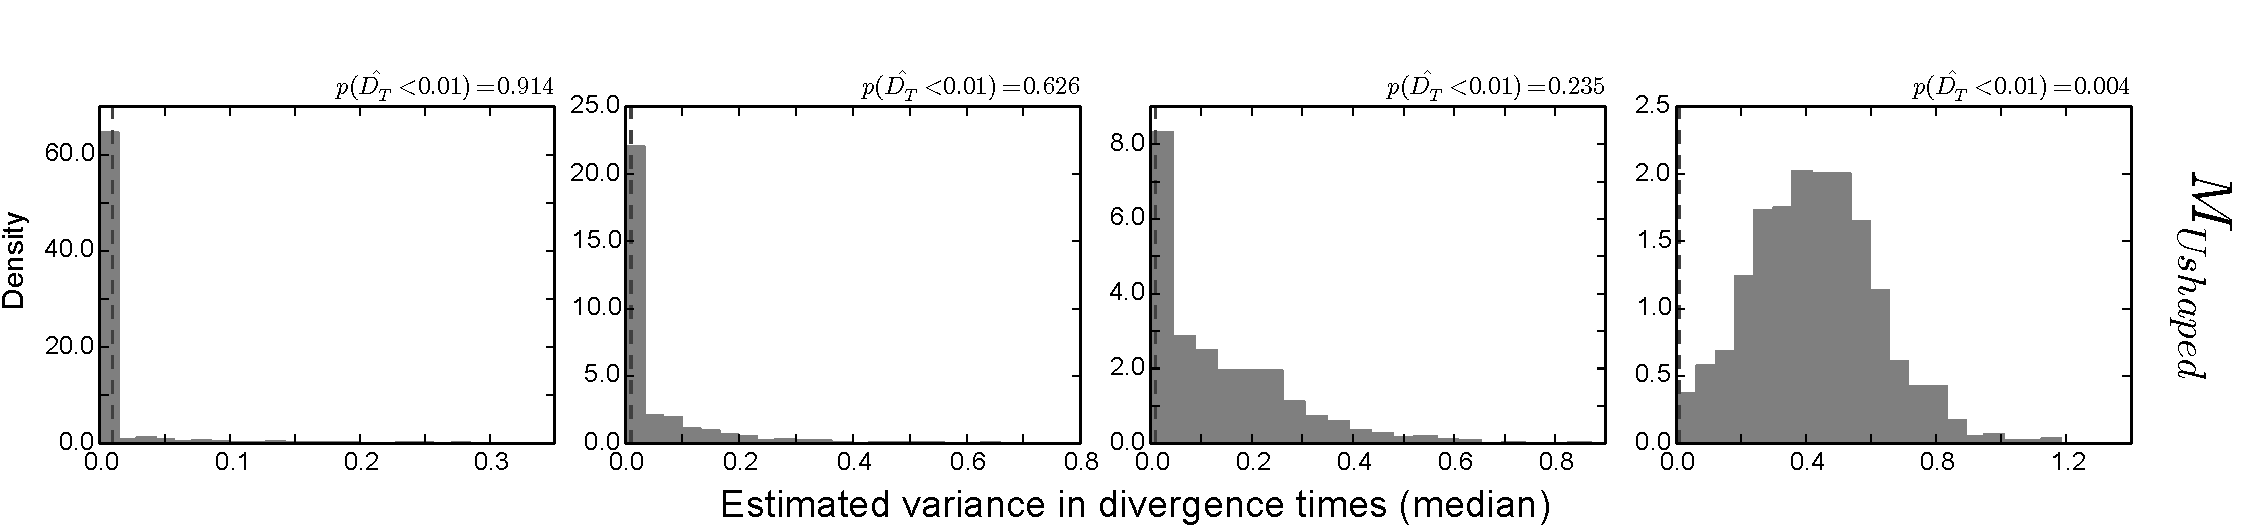
\includegraphics[width=\textwidth]{../images/old_u-shaped_power_omega_median_headless.pdf}}
        \vspace{0mm}
        \centerline{
        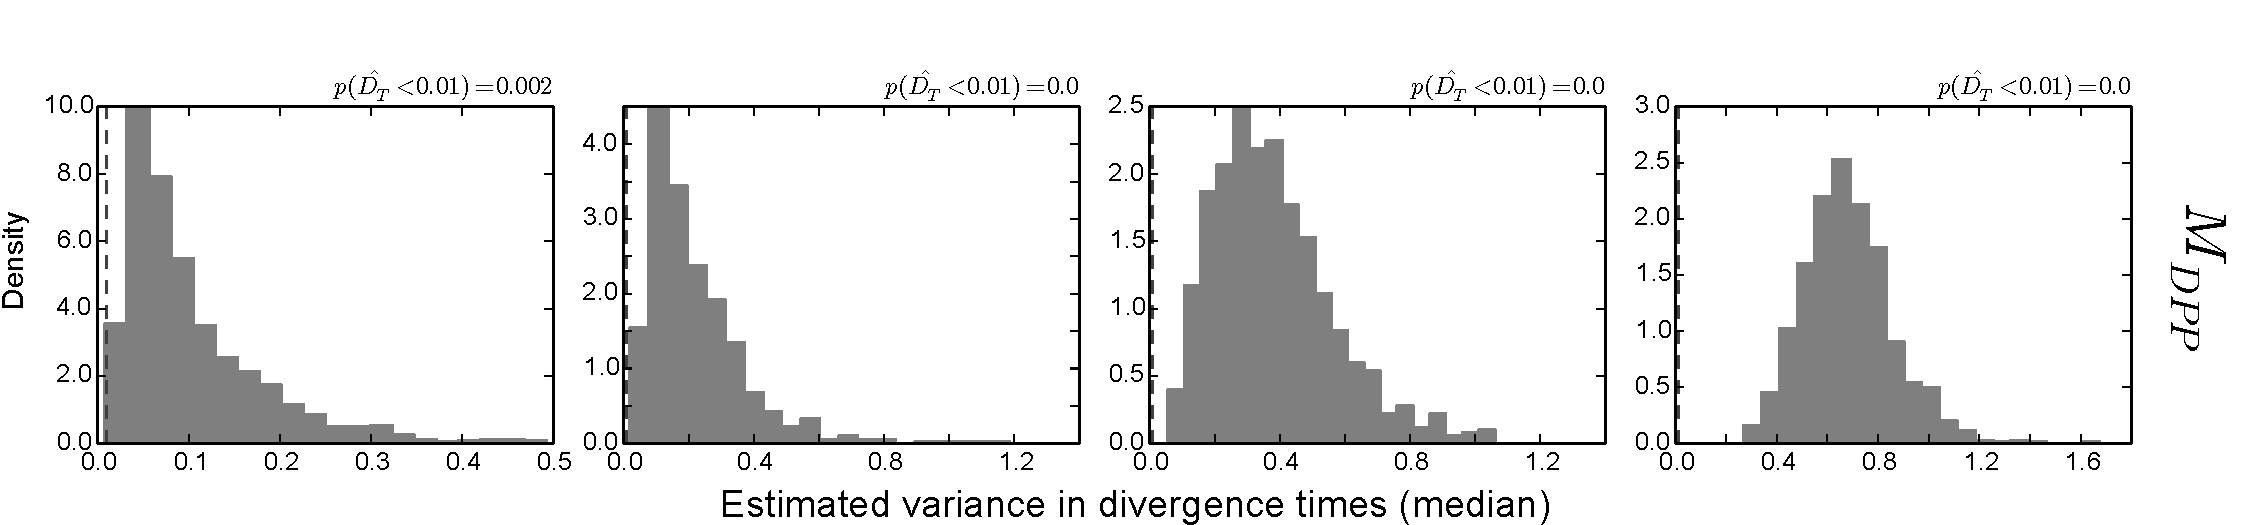
\includegraphics[width=\textwidth]{../images/old_dpp_power_omega_median_headless.pdf}}
    % \barefootnote{\shortfullcite{Oaks2014dpp}}
\end{frame}


\end{document}

